\chapter{分数视角：从 EBM 到 NCSN}\label{ch:score-based}

% In the previous chapters we traced diffusion models back to their variational roots, showing how they emerge from the framework of VAEs. We now turn to a second, equally fundamental view-point: \emph{Energy-Based Models (EBMs)}. EBMs describe data distributions through unnormalized energy functions, and by examining their gradients we arrive at the notion of a \emph{score function}. This chapter builds the bridge from EBMs to what will later crystallize as \emph{score-based diffusion models}. For readers already versed in EBMs, this section serves as a focused refresher and a stepping stone toward the score-based view.

在前几章中，我们将扩散模型追溯到其变分根源，并展示了它们如何在 VAE 的框架内产生。现在我们转向第二个同样基本的视角：\emph{基于能量的模型}（EBM）~\citep{ackley1985learning,lecun2006tutorial}。EBM 通过一个能量景观来表示分布：该景观在数据处能量低，在别处能量高。采样通常依赖于 Langevin 动力学，它通过沿着该景观的梯度移动样本，将其引向高密度区域。这个梯度场被称为\emph{分数}（score），指向概率更高的方向。

核心观察是：仅知道分数就足以进行生成——它能将样本移向高概率区域，而无需计算难以处理的归一化常数。\emph{基于分数的}扩散模型直接建立在这一思想之上。它们不再只关注干净的数据分布，而是考虑一系列被高斯噪声扰动的分布，这些分布的分数更易于近似。学习这些分数得到一族向量场，它们逐步引导带噪样本回归到数据，从而把生成转化为渐进式去噪。




% \se{fix language, ideally give some intuition for this connection}

\newpage


\section{基于能量的模型}\label{sec:ebm}

对于已经熟悉 EBM 的读者，本节作为一个简明的回顾，并作为通向扩散模型分数视角的桥梁。
\subsection{使用能量函数建模概率分布}

设 $\mathbf{x} \in \mathbb{R}^D$ 表示一个数据点。EBM 通过由 ${\bm{\phi}}$ 参数化的能量函数 $E_{\bm{\phi}}(\mathbf{x})$ 定义概率密度，该函数为更可能的配置赋予更低的能量。所得分布为
\begin{align*}
    p_{{\bm{\phi}}}(\mathbf{x}) := \frac{\exp(-E_{\bm{\phi}}(\mathbf{x}))}{Z_\bphi}, \quad 
    Z_\bphi := \int_{\mathbb{R}^D} \exp(-E_{\bm{\phi}}(\mathbf{x})) \diff\mathbf{x},
\end{align*}
其中 $Z_\bphi$ 称为\emph{配分函数}，用于保证归一化：
\[
\int_{\mathbb{R}^D} p_{{\bm{\phi}}}(\mathbf{x})  \diff\mathbf{x} = 1.
\]
\begin{figure}[th!]
    \centering
    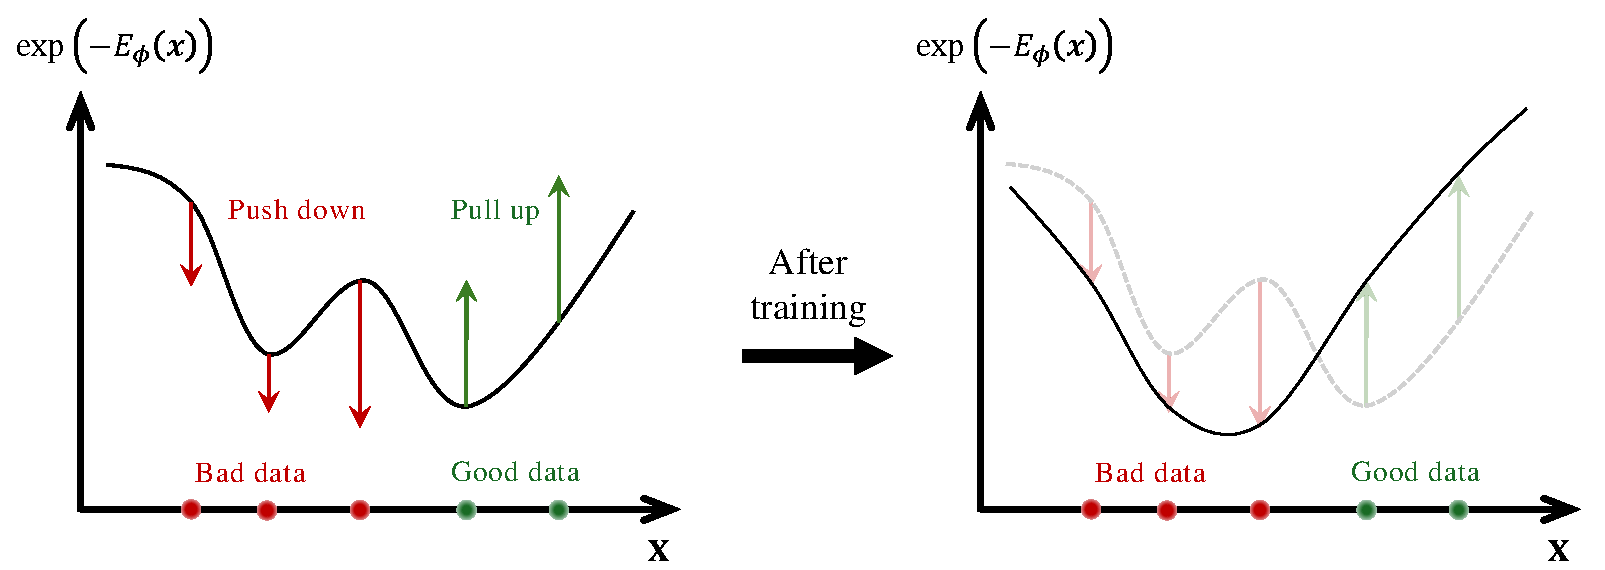
\includegraphics[width=\linewidth]{Images/PartB/ebm-graph.pdf}
    \caption{\textbfs{EBM 训练示意图。} 模型在``坏''数据点处降低密度（升高能量）（红色箭头），并在``好''数据点处升高密度（降低能量）（绿色箭头）。 \figcredit{由作者绘制。}}
    \label{fig:ebm-graph}
\end{figure}



在这种视角下，能量更低的点对应更高的概率，就像一个球滚入山谷一样。配分函数 $Z_{\bphi}$ 确保所有概率之和为一，因此只有能量的\emph{相对}值才起作用。例如，给所有能量加上一个常数会使分子和分母同乘相同的因子，分布保持不变。

此外，由于配分函数 $Z_{\bphi}$ 强制概率之和为一，从数学上可知，降低某一区域内的能量会增加其概率，而其补集的概率则相应减少。因此，EBM 遵循严格的全局权衡：使一个山谷更深必然会使其他山谷变浅，概率质量在整个空间上被重新分配，而非独立地分配给每个区域。


\paragraph{EBM 中极大似然训练的挑战。}
原则上，EBM 可以通过极大似然来训练，这种方法自然地在拟合数据与全局正则化之间取得平衡（见 \Cref{eq:MLE}）：
\begin{align}
\label{eq:mle-ebm}
\mathcal{L}_{\text{MLE}}(\bphi) 
&= \mathbb{E}_{p_{\text{data}}(\rvx)}  \left[ \log \frac{\exp(-E_{\bphi}(\rvx))}{Z_\bphi} \right] \\
&= -  \underbrace{\mathbb{E}_{p_{\text{data}}}[E_{\bphi}(\rvx)]}_{\text{lowers energy of data}}
   -  \underbrace{\log \int \exp(-E_{\bphi}(\rvx))\diff\rvx}_{\text{global regularization}}, \nonumber
\end{align}
其中 $Z_\bphi = \int \exp(-E_\bphi(\rvx))\diff\rvx$。
第一项降低真实数据的能量，而第二项通过配分函数强制归一化。

然而，在高维情形下，计算 $\log Z_{\bphi}$ 及其梯度是难以处理的，因为它需要在模型分布下求期望。
这促使人们寻找替代目标：要么近似该项，例如对比散度\citep{hinton2002training}；要么通过\emph{分数匹配}完全绕开它。

接下来，我们首先在 \Cref{subsec:motivation-score} 中介绍分数函数的概念，并在 \Cref{subsec:training-ebm} 中将分数匹配作为绕开配分函数的可处理训练目标加以介绍，然后在 \Cref{subsec:sampling-ebm} 中讨论将 Langevin 动力学作为一种实用的、基于分数函数的采样方法。

% \paragraph{Preface: Efficient EBM Training via Score Matching.}


% \paragraph{Preface: Sampling via Score Functions.}
% Training alone is not sufficient; EBMs must also generate samples from their learned energy landscape. 
% Since they lack an explicit generator, this is typically achieved with Markov Chain Monte Carlo methods. 
% Among these, \emph{Langevin dynamics} is particularly effective: it updates samples using only the gradient of the energy (the score function), 
% guiding them toward regions of higher probability and enabling efficient sampling without computing the partition function.













% \paragraph{Intuition Behind Energy-Based Models.}
% \jcr{Drawing from the physical analogy of a ball gravitating towards a low-energy valley, Energy-Based Models (EBMs) define a distribution by assigning an \emph{energy} $E_\bphi(\rvx)$ to each point $\rvx$ and converting these values into probabilities $p_\bphi(\rvx) = \tfrac{\exp(-E_\bphi(\rvx))}{Z_\bphi}$. Lower energy means larger $\exp(-E_\bphi(\rvx))$ and thus higher probability mass, so regions where the energy landscape forms deep valleys correspond to more likely and realistic data. The partition function $Z_\bphi$ ensures proper normalization, since $\exp(-E_\bphi(\rvx))$ alone does not integrate to one. Importantly, only relative energies matter: adding a constant $c$ shifts both numerator and denominator by the same factor $e^{-c}$, leaving $p_\bphi$ unchanged.

% This normalization induces a global trade-off across the space. To see this, consider a region $A$, where its probability under $p_\bphi$ is
% \[
% \frac{\int_A \exp(-E_\bphi(\rvx)) \diff\rvx}{\int \exp(-E_\bphi(\rvx)) \diff\rvx} = \frac{\int_A \exp(-E_\bphi(\rvx)) \diff\rvx}{\int \exp(-E_\bphi(\rvx)) \diff\rvx}.
% \]
% If $E_\bphi$ is decreased on $A$, the numerator grows and thus the probability on $A$ increases. Since the denominator grows as well, the relative weight of the complement $A^c$ must shrink so that the total probability remains one. In plain words, making one valley deeper necessarily makes other valleys shallower, because $Z_\bphi$ redistributes probability mass across the entire space. This captures the essence of EBMs: the model does not assign probabilities independently to regions, but balances them through a single global normalization.

% }
% % Drawing from the physical notion that systems gravitate towards lower potential energy (e.g., a ball in a valley), Energy-Based Models define a probability distribution by assigning an \emph{energy} $E_\bphi(\mathbf{x})$ to each data point $\mathbf{x}$. Crucially, lower energy corresponds to higher likelihood and more realistic data, while high energy signals low probability, mirroring how physical systems avoid high-energy configurations. This framework allows EBMs to model intricate, multimodal distributions without explicit latent variables or restrictive parametric assumptions, distinguishing them from approaches like VAEs. 
% % The energy function provides a direct, interpretable measure of data plausibility.
% % \se{won't be clear why without mentioning normalization}

% % \se{need to add citations}



% \paragraph{Challenge of Energy-Based Models.}
% Despite their conceptual appeal, EBMs are challenging to train (and actually also sample) due to the intractability of $Z_\bphi$, which involves integrating over the full input space. Consequently, practical methods rely on approximate or surrogate objectives that bypass direct evaluation of the partition function while still encouraging the model to fit the data distribution.


% \paragraph{Naïve Training of Energy-Based Models.}
% \jc{The fundamental goal when training an EBM is to assign low energy to genuine data points, making them highly probable under our model. In theory, one could drive the energy of training samples arbitrarily low, leading to a degenerate `spiky'' density that places almost all probability on the data and ignores the rest of the space. In practice, however, this collapse is prevented by the smooth and finite capacity parameterization of a neural network $E_\bphi$, which, together with the global normalization constraint, discourages sharply concentrated distributions.
% }
% \se{not sure this overfitting discussion is valuable here}
% This trade-off is naturally captured by the maximum likelihood objective (see \Cref{eq:MLE}), which balances data fitting with global regularization:
% \begin{align}
% \begin{aligned}
%     \label{eq:mle-ebm}
%     \mathcal{L}_{\text{MLE}}({\bm{\phi}}) &= \mathbb{E}_{p_{\text{data}}(\mathbf{x})} \left[ \log \frac{\exp(-E_{\bm{\phi}}(\rvx))}{Z_\bphi} \right] \\
%     &= - \underbrace{\mathbb{E}_{p_{\text{data}}(\mathbf{x})} [E_{\bm{\phi}}(\rvx)]}_{\text{pulls down energy of data}} - \underbrace{\log \int_{\mathbb{R}^D} \exp(-E_{\bm{\phi}}(\mathbf{x})) \diff\mathbf{x}}_{\text{global regularization}},
% \end{aligned}
% \end{align}
% where we use the definition of $Z_\bphi=\int \exp(-E_\bphi(\rvx))\diff\rvx$.
% % \se{probably better to spell out the def of the partition function here (integral) so the tradeoff is clear}
% The first term encourages low energy for real samples, while the second term, via the partition function $Z_\bphi$, penalizes spreading low energy too broadly; thus promoting a well-distributed model.

% % However, computing $Z_\bphi$ is generally intractable, as it involves integrating over the entire data space. Consequently, exact maximum likelihood training is rarely feasible in practice. This motivates the use of approximation methods such as \emph{Contrastive Divergence} or alternative objectives like \emph{Score Matching}, which offer tractable estimates of the gradient. \se{add citations. tie to the divergence discussion in early chapters?}


% \jcr{
% While conceptually simple, evaluating the partition function $Z_\bphi$ is typically intractable because it integrates over the entire space, which makes exact maximum likelihood impractical. Classical approximations such as contrastive divergence~\citep{hinton2002training}, but here we emphasize score matching~\citep{hyvarinen2005estimation}, which replaces likelihood training with the Fisher divergence discussed earlier in \Cref{eq:fisher}. Crucially, this objective avoids $Z_\bphi$ because the score does not depend on the normalization constant. 
% }


% Sampling from EBMs poses another key challenge. Unlike models with explicit decoders, EBMs define only an energy landscape. To generate samples, we typically resort to \emph{Markov Chain Monte Carlo (MCMC)} methods. Unfortunately, many standard MCMC techniques require full likelihood evaluations \se{i don't think that's true, which one are you thinking about?}, which again involve $Z_\bphi$. A widely used workaround is \emph{Langevin Dynamics}, which leverages the gradient of the energy function alone. This allows us to sample effectively from the learned distribution without evaluating the full normalization constant.

% We first discuss in details score matching training technique of EBMs that bypass the need for exact likelihoods, and subsequently move to Langevin Dynamics as a practical sampler.

% \se{this setup training-inference-training is messy}


% \subsection{Motivation--What Is Score?}\label{subsec:motivation-score}

% We begin by formally defining the score function~\citep{stein1972bound}. For a probability density function $ p(\rvx) $ on $ \mathbb{R}^D $, the \emph{score function} is the vector field given by the gradient of the log-density:
% \[
% \rvs(\rvx) := \nabla_{\rvx} \log p(\rvx),
% \]
% where $ \rvs \colon \mathbb{R}^D \to \mathbb{R}^D $.

% The score function can be understood as the gradient field of a probability landscape. Instead of describing absolute likelihoods, it points locally in the direction where probability increases most steeply, thus offering an intuitive and mathematically precise guide for navigating toward regions of higher data density.

% \begin{figure}[th]
%     \centering
%     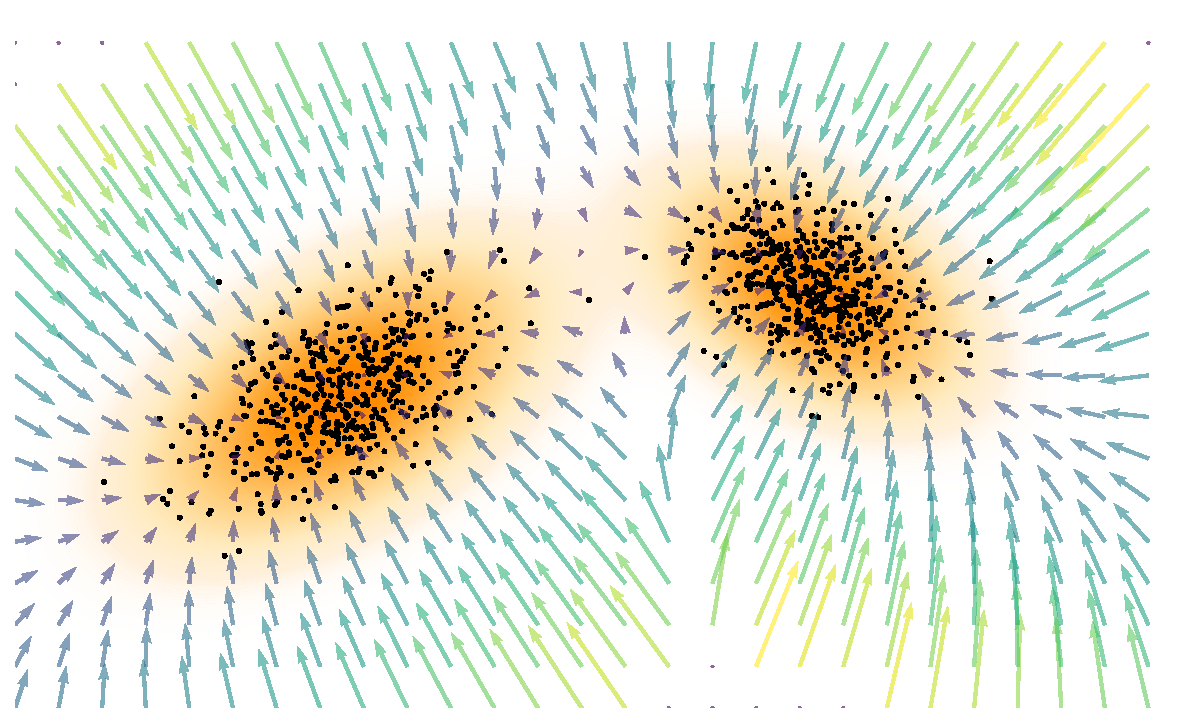
\includegraphics[width=0.95\linewidth]{Images/PartB/score_function_plot.pdf}
%     \caption{Visualization of score vector fields $\nabla_{\rvx} \log p(\rvx)$, which indicate the direction of increasing probability density under $p(\rvx)$.}
%     \label{fig:score-function}
% \end{figure}

% \paragraph{Why the Score Function Excels?}
% \jcr{A natural question arises: why model the score function instead of the probability distribution directly?
% The score provides both theoretical clarity and practical benefits. We start by outlining its conceptual foundations and will highlight further advantages as the chapter unfolds.}
% % One may question the rationale behind modeling the score function rather than the probability distribution itself.
% % \se{fix language. also transition to this paragraph is very rough, this was not mentioned before}
% % Indeed, the score function offers both theoretical and practical advantages. We begin by introducing its conceptual foundations and will progressively highlight additional benefits throughout this chapter.

% \subparagraph{1. Freedom from Normalization Constants.}
% Many distributions are defined only up to an unnormalized density $\tilde{p}(\rvx)$, e.g., $\exp(-E_{\bm{\phi}}(\rvx))$ in EBMs with
% \[
% p(\rvx) = \frac{\tilde{p}(\rvx)}{Z}, 
% \qquad 
% Z = \int \tilde{p}(\rvx)  \diff\rvx.
% \]
% Evaluating $Z_{\bm{\phi}}$ is generally intractable, creating a bottleneck for training.  
% The score function removes this difficulty:
% \begin{align}\label{eq:score-no-constant}
%     \nabla_{\rvx}\log p(\rvx) 
% = \nabla_{\rvx}\log \tilde{p}(\rvx) - \underbrace{\nabla_{\rvx}\log Z}_{=0}
% = \nabla_{\rvx}\log \tilde{p}(\rvx),
% \end{align}
% since $Z$ is constant in $\rvx$.  
% Hence the score depends only on $\tilde{p}$, allowing EBMs to be trained without computing $Z$.



% \subparagraph{2. A Complete and Expressive Representation.}
% Focusing on the score function does not entail any loss of information about the original distribution. The score function uniquely characterizes the distribution since it is the gradient of the log-density. Conversely, the original density can be recovered from the score function up to a constant:
% \[
% \log p(\rvx) = \log p(\rvx_0) + \int_0^1 \rvs(\rvx_0 + t(\rvx - \rvx_0))^\top (\rvx - \rvx_0)  \diff t,
% \]
% where $\rvx_0$ is a reference point and $\log p(\rvx_0)$ acts as an integration constant fixed by normalization. This equivalence establishes that modeling the score function is as expressive as modeling the density itself, offering a tractable alternative for generative modeling.




% \subsection{Training EBMs with Score Matching}\label{subsec:training-ebm}
% % \paragraph{Contrastive Divergence.} 
% % \se{should we cut this? not sure it's relevant}
% % One challenge in training EBMs is the difficulty of sampling from the model. A widely used workaround is \textit{Contrastive Divergence}, which approximates model samples using short-run MCMC.

% % We revisit \Cref{eq:mle-ebm}. Taking the gradient of the MLE objective with respect to $\bm{\phi}$ yields:
% % \begin{align*}
% %     &\nabla_{\bm{\phi}} \mathcal{L}_{\text{MLE}}(\bm{\phi}) \\
% %     =&\mathbb{E}_{p_{\text{data}}(\mathbf{x})} [-\nabla_{\bm{\phi}}E_{\bm{\phi}}(\rvx)] - \mathbb{E}_{p_{{\bm{\phi}}}(\mathbf{x})} [\nabla_{\bm{\phi}}\log Z_\bphi]\\
% %     =&\mathbb{E}_{p_{\text{data}}(\mathbf{x})} [-\nabla_{\bm{\phi}}E_{\bm{\phi}}(\rvx)] - \mathbb{E}_{p_{{\bm{\phi}}}(\mathbf{x})} \left[\frac{1}{Z_\bphi} \int \nabla_{\bm{\phi}} \exp(-E_{\bm{\phi}}(\rvx))    \diff\mathbf{x}\right]\\
% % = &\mathbb{E}_{p_{\text{data}}(\mathbf{x})} \left[ -\nabla_{\bm{\phi}} E_{\bm{\phi}}(\rvx) \right]
% % + \mathbb{E}_{p_{\bm{\phi}}(\mathbf{x})} \left[ \nabla_{\bm{\phi}} E_{\bm{\phi}}(\rvx) \right].
% % \end{align*}
% % This motivates the CD loss:
% % \begin{align}\label{eq:contrastive-div}
% %     \mathcal{L}_{\text{CD}}({\bm{\phi}}) 
% % = \mathbb{E}_{p_{\text{data}}(\mathbf{x})} [E_{\bm{\phi}}(\rvx)] 
% % - \mathbb{E}_{\tilde{p}_{{\bm{\phi}}}(\mathbf{x})} [E_{\bm{\phi}}(\rvx)],
% % \end{align}
% % where $\tilde{p}_{\bm{\phi}}(\mathbf{x})$ is an approximate distribution obtained by running a few MCMC steps (e.g., Langevin dynamics) initialized from a data point. This objective approximates the MLE gradient without requiring full convergence of the Markov chain. However, it still incurs computational cost due to the need to simulate MCMC at each training step.

% Maximum likelihood training of EBMs is difficult because of the partition function. 
% \emph{Score matching}~\citep{hyvarinen2005estimation} provides a practical alternative: rather than fitting normalized probabilities, 
% it aligns the score of the model with those of the data.  
% Since these gradients depend only on the energy function, score matching completely bypasses the partition function as we showed in \Cref{eq:score-no-constant}:
% \jcr{
% \begin{align*}
%     \nabla_{\mathbf{x}} \log p_{\bm{\phi}}(\mathbf{x}) &= \nabla_{\mathbf{x}} \log \frac{\exp(-E_{\bm{\phi}}(\rvx))}{Z_\bphi} \\ &= - \nabla_{\mathbf{x}} E_{\bm{\phi}}(\mathbf{x}) - \underbrace{\nabla_{\mathbf{x}} \log Z_\bphi}_{=0} \\&= - \nabla_{\mathbf{x}} E_{\bm{\phi}}(\mathbf{x}) ,
% \end{align*}
% }
% The score matching objective minimizes the discrepancy between the model's score and the (unknown) data score:
% \begin{align}\label{eq:ebm-sm}
% \mathcal{L}_{\mathrm{SM}}(\bm{\phi}) := \mathbb{E}_{p_{\mathrm{data}}(\mathbf{x})} \left[ \frac{1}{2} \left\| \nabla_{\mathbf{x}} \log p_{\bm{\phi}}(\mathbf{x}) - \nabla_{\mathbf{x}} \log p_{\mathrm{data}}(\mathbf{x}) \right\|_2^2 \right].
% \end{align}
% \paragraph{Score Matching: An Alternative Objective.}
% When the true data score $\nabla_{\mathbf{x}} \log p_{\mathrm{data}}(\mathbf{x})$ is inaccessible, score matching offers an ingenious alternative. Under mild regularity conditions (e.g., vanishing boundary terms), its objective can be elegantly reformulated using integration by parts (see Proposition~\ref{sm-trace}):
% \begin{align*}
% \mathcal{L}_{\mathrm{SM}}(\bm{\phi})
% = \mathbb{E}_{p_{\mathrm{data}}(\mathbf{x})} \left[
% \Tr\left(\nabla_{\mathbf{x}}^2 E_{\bm{\phi}}(\rvx) \right)
% + \frac{1}{2} \left\| \nabla_{\mathbf{x}} E_{\bm{\phi}}(\rvx) \right\|_2^2
% \right] + C,
% \end{align*}
% where $\nabla_{\mathbf{x}}^2 E_{\bm{\phi}}(\rvx)$ denotes the Hessian of $E_{\bm{\phi}}$ with respect to $\mathbf{x}$, and $C$ is a constant independent of $\bm{\phi}$.
% This formulation is particularly appealing because it removes the need to compute the intractable partition function $Z_\bphi$ and avoids costly sampling from the model distribution during training. Nevertheless, score matching introduces its own challenges. Specifically, the requirement to compute second-order derivatives (Hessians) often becomes computationally prohibitive, especially in high-dimensional settings.


\subsection{动机：什么是分数？}\label{subsec:motivation-score}

对于 $\mathbb{R}^D$ 上的密度 $p(\rvx)$，\emph{分数函数}是对数密度的梯度：
\[
\rvs(\rvx) := \nabla_{\rvx} \log p(\rvx), \qquad \rvs \colon \mathbb{R}^D \to \mathbb{R}^D.
\]
直观上，分数构成一个指向更高概率区域的向量场，为数据最可能出现的位置提供局部指引（见 \Cref{fig:score-function}）。

\begin{figure}[th]
    \centering
    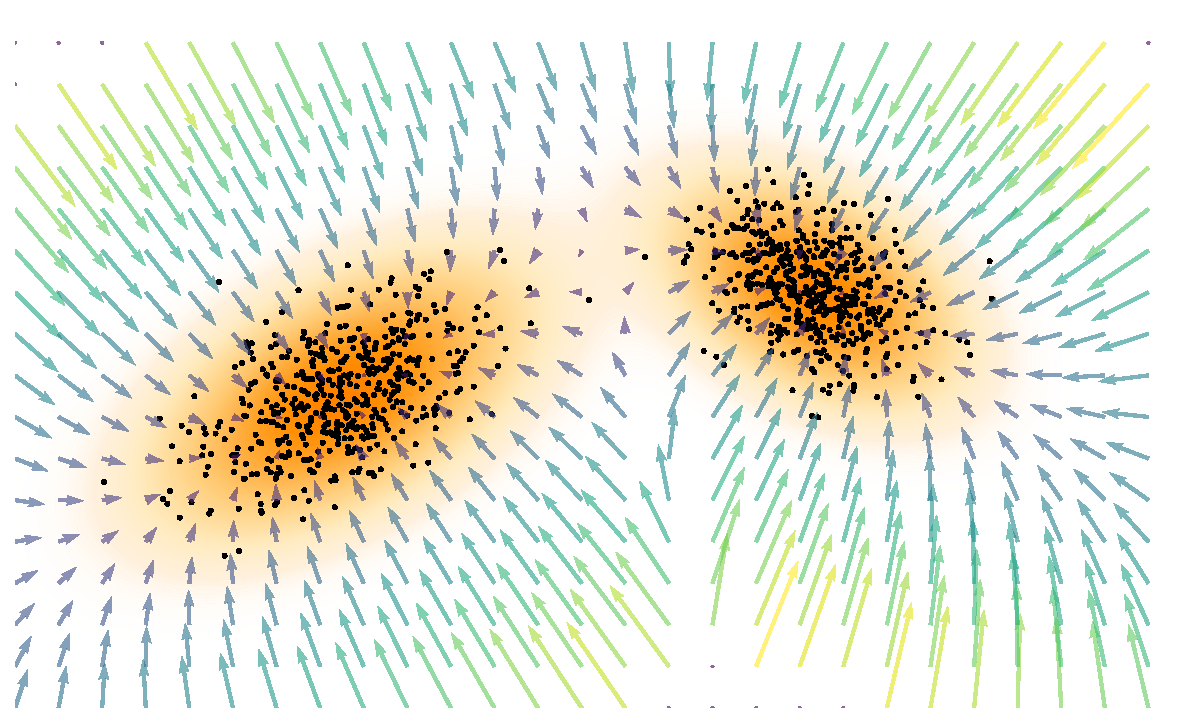
\includegraphics[width=0.95\linewidth]{Images/PartB/score_function_plot.pdf}
    \caption{\textbfs{分数向量场示意图。} 分数向量场 $\nabla_{\rvx} \log p(\rvx)$ 指示密度增加的方向。 \figcredit{由作者绘制。}}
    \label{fig:score-function}
\end{figure}

\paragraph{为什么要建模分数而非密度？}
建模分数在理论和实践上都有优势：


\subparagraph{1. 摆脱归一化常数。}
    许多分布只定义到未归一化密度 $\tilde{p}(\rvx)$，例如 EBM 中的 $\exp(-E_{\bm{\phi}}(\rvx))$：
    \[
    p(\rvx) = \frac{\tilde{p}(\rvx)}{Z}, 
    \qquad 
    Z = \int \tilde{p}(\rvx)\diff\rvx.
    \]
    虽然计算 $Z$ 是难以处理的，但分数只依赖于 $\tilde{p}$：
\begin{align}\label{eq:score-compute}
\nabla_{\rvx}\log p(\rvx) = \nabla_{\rvx}\log \tilde{p}(\rvx) - \underbrace{\nabla_{\rvx}\log Z}_{=0} = \nabla_{\rvx}\log \tilde{p}(\rvx), \end{align} 
因为 $Z$ 关于 $\rvx$ 是常数。这完全绕开了配分函数。

\subparagraph{2. 完整的表示。}
分数函数完整地刻画了底层分布。
由于它是对数密度的梯度，因此密度可以（相差一个常数）通过下式恢复：
\[
\log p(\rvx) 
= \log p(\rvx_0) + \int_0^1 \rvs(\rvx_0 + t(\rvx - \rvx_0))^\top (\rvx - \rvx_0)  \diff t,
\]
其中 $\rvx_0$ 是参考点，$\log p(\rvx_0)$ 由归一化确定。
因此，建模分数与建模 $p(\rvx)$ 本身一样富有表现力，同时在生成建模中往往更易处理。


\subsection{通过分数匹配训练 EBM}\label{subsec:training-ebm}
在 EBM 中，密度定义为 $p_{{\bm{\phi}}}(\mathbf{x}) = \tfrac{\exp(-E_{\bm{\phi}}(\mathbf{x}))}{Z_\bphi}$。极大似然训练需要计算 $Z_{\bm{\phi}}$，而这通常是难以处理的。
一个关键观察是：$p_{{\bm{\phi}}}$ 的模型分数简化为 $-\nabla_{\rvx}E_{\bm{\phi}}(\rvx)$，与 $Z_{\bm{\phi}}$ 无关（见 \Cref{eq:score-compute}）。

\emph{分数匹配}~\citep{hyvarinen2005estimation} 利用了分数只依赖于能量函数这一事实。
它不再拟合归一化概率，而是通过对齐模型分数与（未知的）数据分数来训练 EBM：
\begin{align}\label{eq:ebm-sm}
    \mathcal{L}_{\mathrm{SM}}(\bm{\phi}) 
= \tfrac{1}{2}  \mathbb{E}_{p_{\mathrm{data}}(\mathbf{x})} 
\big\| \nabla_{\mathbf{x}} \log p_{\bm{\phi}}(\mathbf{x}) 
- \nabla_{\mathbf{x}} \log p_{\mathrm{data}}(\mathbf{x}) \big\|_2^2.
\end{align}

尽管数据分数不可得，但分部积分可以得到一个仅涉及能量及其导数的等价表达式（详见命题~\ref{sm-trace}）：
\[
\mathcal{L}_{\mathrm{SM}}(\bm{\phi}) =
\mathbb{E}_{p_{\mathrm{data}}(\mathbf{x})} \left[
-\Tr \big(\nabla_{\mathbf{x}}^2 E_{\bm{\phi}}(\rvx)\big)
+ \tfrac{1}{2}  \|\nabla_{\mathbf{x}} E_{\bm{\phi}}(\rvx)\|_2^2
\right] + C,
\]
其中 $\nabla_{\mathbf{x}}^2 E_{\bm{\phi}}(\rvx)$ 是 $E_{\bm{\phi}}$ 的 Hessian 矩阵，$C$ 是与 $\bm{\phi}$ 无关的常数。

这一表述很有吸引力，因为它消除了配分函数，并避免了在训练过程中从模型中采样。
它的主要缺点是需要二阶导数：尽管只需要 Hessian 矩阵的迹（$\Tr \big(\nabla_{\mathbf{x}}^2 E_{\bm{\phi}}\big)$），而非完整的 Hessian 矩阵，但该项的精确计算通常需要跨输入坐标汇总二阶导数信息，因此其代价通常随输入维度 $D$ 的增加而上升。
我们将在本章后面重新讨论解决该局限的方法。






\subsection{基于分数函数的 Langevin 采样}\label{subsec:sampling-ebm}
从由能量函数 $E_{\bm{\phi}}(\mathbf{x})$ 定义的 EBM 中采样，可以使用\emph{Langevin 动力学}来完成。我们首先介绍离散时间的 Langevin 更新，然后介绍其作为随机微分方程（SDE）的连续时间极限。最后，我们讨论 Langevin 动力学如何实现对复杂能量景观高效探索的物理直觉。


\begin{figure}
    \centering
    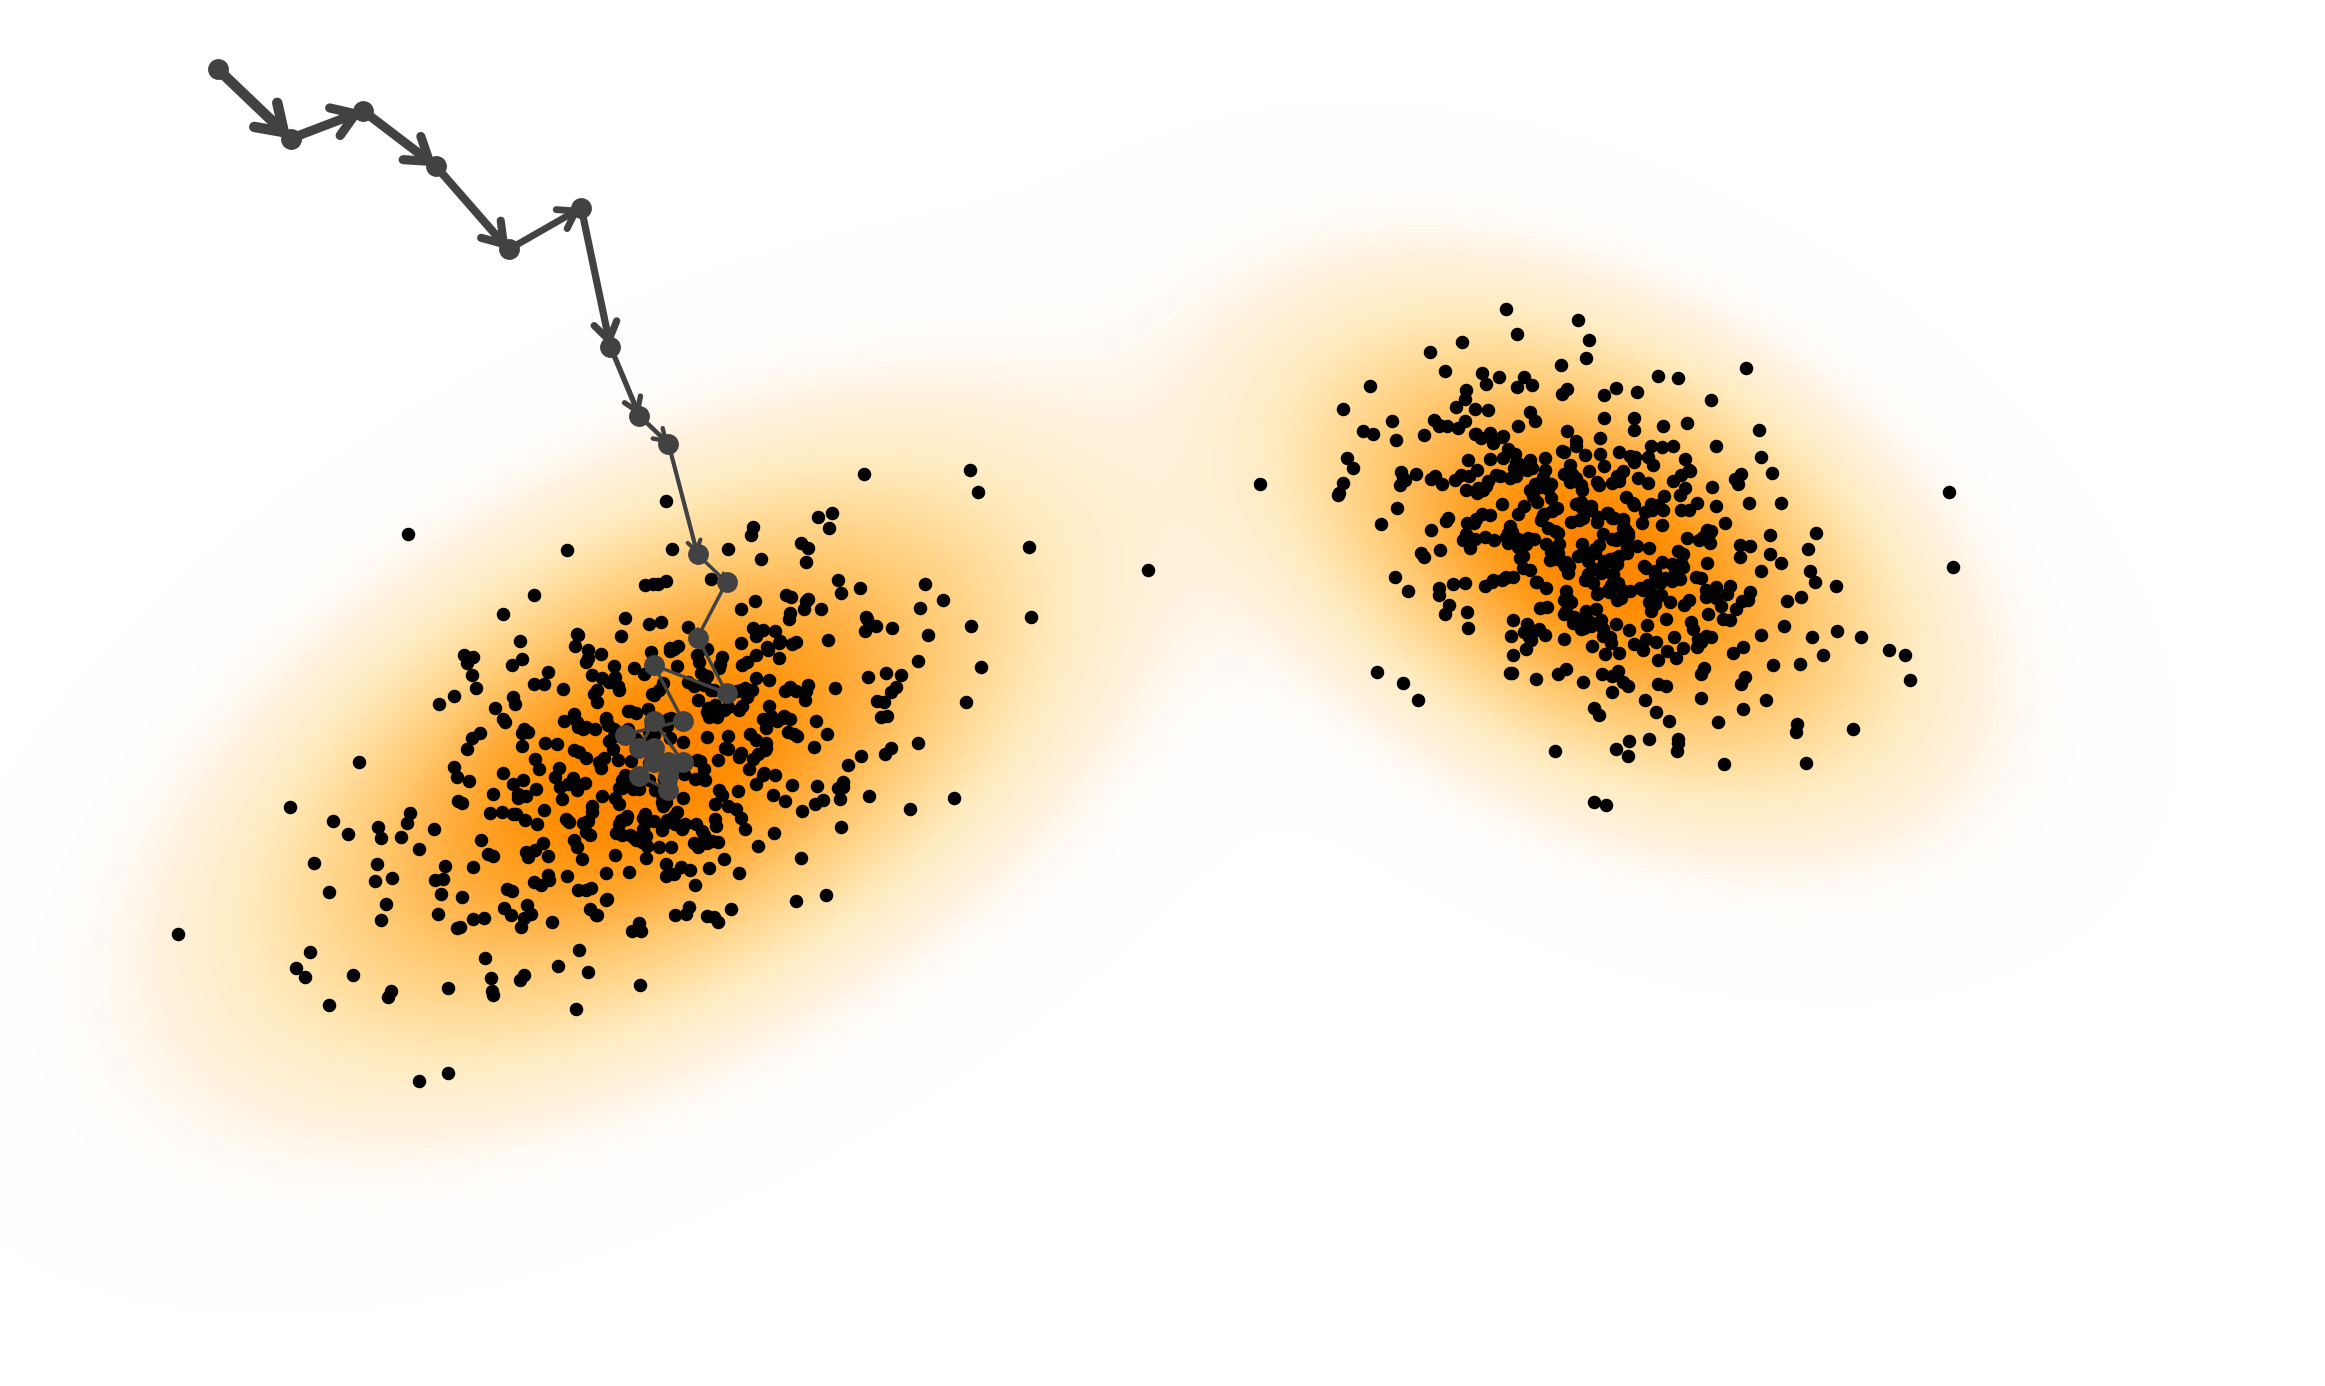
\includegraphics[width=\linewidth]{Images/PartB/langevin_sampling.png}
    \vspace{-1.5cm}
    \caption{\textbfs{Langevin 采样示意图。} Langevin 采样利用分数函数 $\nabla_{\mathbf{x}} \log p_{\bm{\phi}}(\mathbf{x})$，通过 \Cref{eq:discrete-langevin-score} 中的更新（以箭头表示）引导轨迹走向高密度区域。 \figcredit{由作者绘制。}}
    \label{fig:langevin}
\end{figure}


\paragraph{离散时间 Langevin 动力学。}
离散时间的 Langevin 更新为
\begin{align}\label{eq:discrete-langevin}
    \mathbf{x}_{n+1} = \mathbf{x}_n - \eta \nabla_{\mathbf{x}} E_{\bm{\phi}}(\mathbf{x}_n) +  \sqrt{2 \eta} \bm{\epsilon}_n, \quad n=0,1,2,\ldots,
\end{align}
其中 $\mathbf{x}_0$ 由某个分布（通常是高斯分布）初始化，$\eta > 0$ 是步长，$\bm{\epsilon}_n \sim \mathcal{N}(\mathbf{0}, \mathbf{I})$ 是高斯噪声。噪声通过引入随机性使得探索能够超越局部极小值。

由于分数函数可以计算为
\[
\nabla_{\mathbf{x}} \log p_{\bm{\phi}}(\mathbf{x}) = -\nabla_{\mathbf{x}} E_{\bm{\phi}}(\rvx).
\]
% \se{important to show why partition function disappears}
该更新可以等价地写为
\begin{align}\label{eq:discrete-langevin-score}
    \mathbf{x}_{n+1} = \mathbf{x}_n + \eta \nabla_{\mathbf{x}} \log p_{\bm{\phi}}(\mathbf{x}_n) + \sqrt{2 \eta}\bm{\epsilon}_n,
\end{align}
其中分数函数引导样本走向高密度区域。这一表述是扩散模型的核心，后文将详述。

\paragraph{连续时间 Langevin 动力学。}
当步长 $\eta$ 趋近于零时，离散 Langevin 更新自然收敛到一个由\emph{Langevin 随机微分方程（SDE）}描述的连续时间过程\footnote{
带有因子 $\sqrt{2}$ 时，Langevin 动力学使 $p_{\bm\phi}$ 不随时间变化。即 $p_{\bm\phi}$ 是平稳的：若 $\rvx(0)\sim p_{\bm\phi}$，则对所有 $t\ge 0$ 都有 $\rvx(t)\sim p_{\bm\phi}$。等价地，$p_{\bm\phi}$ 是 Fokker–Planck 方程的平稳解（见 \Cref{app:continuity}）：
\[
\partial_t \rho = -\nabla \cdot(\rho  \nabla\log p_{\bm\phi}) + \tfrac{\sigma^2}{2}\Delta \rho.
\]
令 $\rho=p_{\bm\phi}$ 得到 $(\tfrac{\sigma^2}{2}-1)\Delta p_{\bm\phi}=0$，仅当 $\sigma=\sqrt{2}$ 时成立。
}
：
\begin{align}\label{eq:continuous-langevin}
 \diff \mathbf{x}(t) = \nabla_{\mathbf{x}} \log p_{\bm{\phi}}(\mathbf{x}(t)) \diff t + \sqrt{2} \diff \mathbf{w}(t),
\end{align}
其中 $\mathbf{w}(t)$ 表示标准布朗运动（也称为 Wiener 过程\footnote{布朗增量满足
$\mathbf{w}(t+\eta)-\mathbf{w}(t)\sim \mathcal{N}(\mathbf{0},  \eta  \mathbf{I})$。
因此 Euler–Maruyama 使用步噪声 $\sqrt{2}  [\mathbf{w}(t+\eta)-\mathbf{w}(t)]
= \sqrt{2\eta}  \bm{\epsilon}_n$，其中 $\bm{\epsilon}_n \sim \mathcal{N}(\mathbf{0},\mathbf{I})$，
这解释了 $\sqrt{\eta}$ 因子；这就是平方根缩放的来源。关于布朗运动和 SDE 的详细介绍，请参阅 \Cref{app:de}.})。需要理解的是，\Cref{eq:discrete-langevin} 中的离散更新规则是这一连续 SDE 的 Euler–Maruyama 离散化。
% \se{will people be confused by the square root on the step size?}


在标准的正则性假设下（例如 $p_{\bm{\phi}}\propto e^{-E_{\bm{\phi}}}$，且 $E_{\bm{\phi}}$ 具有约束性、足够光滑），$\mathbf{x}(t)$ 的分布随 $t\to\infty$（指数级快速）收敛到 $p_{\bm{\phi}}$；因此我们可以通过模拟（求解）SDE \Cref{eq:continuous-langevin} 来采样。



\paragraph{为什么使用 Langevin 采样？}
理解 Langevin 采样的一种自然方式是从物理学视角：能量函数 $ E_{\bm{\phi}}(\mathbf{x}) $ 定义了一个塑造粒子行为的势能景观。根据牛顿动力学，粒子在该能量所导出的力场下的运动由常微分方程（ODE）描述
\[
\diff \mathbf{x}(t) = -\nabla_{\mathbf{x}} E_{\bm{\phi}}\big(\mathbf{x}(t)\big)  \diff t,
\]
它确定性地将粒子沿势能下降方向推向能量函数的局部极小值。然而，这种确定性动力学可能被困在局部极小值中，从而阻碍对完整数据分布的探索。

为克服这一局限，Langevin 动力学引入随机扰动，得到如下 SDE
\[
\diff \mathbf{x}(t) = -\nabla_{\mathbf{x}} E_{\bm{\phi}}\big(\mathbf{x}(t)\big)  \diff t + \underbrace{\sqrt{2 } \diff \rvw(t)}_{\text{injected noise}},
\]
其中 $\rvw(t)$ 是标准布朗运动。
% and $\eta > 0$ is the diffusion coefficient controlling the noise intensity. \se{no diffusion coeff in equation}
噪声项使粒子能够通过越过能量势垒逃出局部极小值，使轨迹成为一个平稳分布收敛到 Boltzmann 分布的随机过程
\[
p_{\bm{\phi}}(\mathbf{x}) \propto e^{-E_{\bm{\phi}}(\mathbf{x})}.
\]

从这个角度看，EBM 可以被视为学习一个力场，它将样本推向高概率区域。Langevin 采样对 EBM 尤为有用，因为它提供了一种实用的方法，能在不显式计算配分函数的情况下从模型分布 $p_{\bm{\phi}}(\mathbf{x})$ 中生成样本。通过迭代地应用 Langevin 更新，可以得到近似目标分布的样本。


\paragraph{Langevin 采样的固有挑战。}
Langevin 动力学作为一种广泛使用的基于马尔可夫链蒙特卡洛（MCMC）的采样器，在高维空间中面临严重局限。其效率对步长 $\eta$、噪声尺度的选择，以及准确近似目标分布所需的迭代次数高度敏感。

这种低效的核心在于``混合时间''过长的问题：在具有许多孤立模态的复杂数据分布中，Langevin 采样通常需要极长时间才能在高概率区域之间转移。这一问题随维度增加而显著恶化，导致收敛速度慢得令人难以承受。

可以把采样想象成在一片广袤崎岖、有许多遥远山谷（每个山谷对应一个不同的数据模态）的景观中探索。Langevin 动力学依赖局部随机更新，难以高效地在这些山谷之间穿行。因此，它往往无法捕捉分布的全部多样性。

这种低效暗示了我们需要更具结构性和引导性的采样方法，以比纯随机探索更有效地在复杂数据流形上游走。



% Secondly, and also fundamentally, score matching primarily constrains the energy function only at the (local) training data points. It fails to impose explicit global regularization on the overall energy landscape, leaving energy values in regions far from training data loosely controlled. This can lead to undesirable or unconstrained model behavior, a crucial difference from directly modeling probability densities. The latter inherently regularizes the entire distribution by implicitly enforcing a global ``sum-to-one'' rule on probabilities, ensuring more stable energy values across the data space.
% \subsection{Closing Remark}
% EBMs and score matching are closely connected. While much research has focused on improving the efficiency and scalability of score matching for training EBMs~\citep{vincent2011connection,song2020sliced}, its role has significantly evolved. Originally developed as an elegant solution to the intractable normalization constant in unnormalized statistical models such as EBMs, score matching has since become a fundamental building block of modern diffusion models. We will explore this important connection in greater detail in the following sections.






\clearpage
\newpage

% \se{the structure of this chapter is unecessarily convoluted. the story is going to be cleaner if you don't mark the background as optional (anyways it's short) and have a coherent story where you have representation, learning, inference. right now therre is too much back and forth between scores, sampling, score matching}


% Consider a landscape representing the probability distribution over data points, where regions of higher elevation correspond to higher likelihoods, and lower regions correspond to lower likelihoods. At each point in this landscape, imagine an arrow indicating the direction of steepest ascent, guiding movement toward areas of increasing probability. This vector field is known as the \emph{score function}~\citep{stein1972bound}, providing an intuitive and precise direction for navigating the probability landscape.


% \subsection{Motivation--What Is Score?}
% We begin by formally defining the score function. For a probability density function $ p(\rvx) $ on $ \mathbb{R}^D $, the \emph{score function} is the vector field given by the gradient of the log-density:
% \[
% \rvs(\rvx) := \nabla_{\rvx} \log p(\rvx),
% \]
% where $ \rvs \colon \mathbb{R}^D \to \mathbb{R}^D $.

% \begin{figure}[th]
%     \centering
%     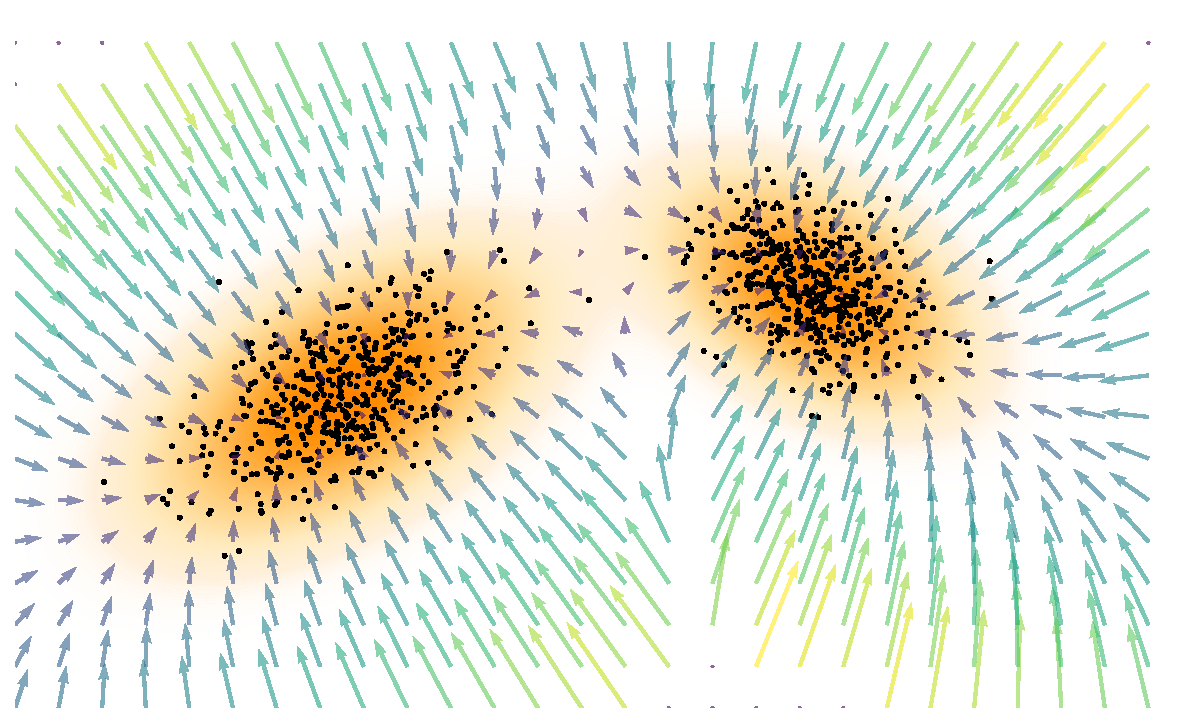
\includegraphics[width=0.95\linewidth]{Images/PartB/score_function_plot.pdf}
%     \caption{Visualization of score vector fields $\nabla_{\rvx} \log p(\rvx)$, which indicate the direction of increasing probability density under $p(\rvx)$.}
%     \label{fig:score-function}
% \end{figure}

% \paragraph{Why the Score Function Excels?}
% One may question the rationale behind modeling the score function rather than the probability distribution itself.
% \se{fix language. also transition to this paragraph is very rough, this was not mentioned before}
% Indeed, the score function offers both theoretical and practical advantages. We begin by introducing its conceptual foundations and will progressively highlight additional benefits throughout this chapter.

% \subparagraph{1. Freedom from Normalization Constants.}
% Many probability distributions are initially defined by an unnormalized density $\tilde{p}(\rvx)$. To turn this into a true probability density $ p(\rvx) $, we must divide by a normalization constant $Z = \int \tilde{p}(\rvx)    \diff \rvx$. Calculating this $Z$ is often computationally prohibitive, involving intractable integrals. This difficulty is a significant bottleneck in training many models, such as EBMs.

% The score function, however, elegantly bypasses this challenge. Consider the derivative:
% \[
% \nabla_{\rvx} \log p(\rvx) = \nabla_{\rvx} \log \left( \frac{\tilde{p}(\rvx)}{Z} \right) = \nabla_{\rvx} \log \tilde{p}(\rvx) - \underbrace{\nabla_{\rvx} \log Z}_{=0}.
% \]
% Since $Z$ is a constant with respect to $ \rvx $, its gradient is zero.
% \[
% \nabla_{\rvx} \log p(\rvx) = \nabla_{\rvx} \log \tilde{p}(\rvx).
% \]
% This remarkable property means the score function is entirely independent of the normalization constant. We can operate directly with unnormalized densities, freeing us from the immense computational burden of computing or approximating $Z$.

% \subparagraph{2. A Complete and Expressive Representation.}
% Focusing on the score function does not entail any loss of information about the original distribution. The score function uniquely characterizes the distribution since it is the gradient of the log-density. Conversely, the original density can be recovered from the score function up to a constant:
% \[
% \log p(\rvx) = \log p(\rvx_0) + \int_0^1 \rvs(\rvx_0 + t(\rvx - \rvx_0))^\top (\rvx - \rvx_0)  \diff t,
% \]
% where $\rvx_0$ is a reference point and $\log p(\rvx_0)$ acts as an integration constant fixed by normalization. This equivalence establishes that modeling the score function is as expressive as modeling the density itself, offering a tractable alternative for generative modeling.



% \paragraph{Using the Score for Generation.}
% Having established that the score function  is a complete and unburdened representation of a distribution, a pivotal question arises:
% \begin{question}
%     Can we actually generate new samples from a complex data distribution if we only know its score function, $ \rvs(\cdot) = \nabla_{\rvx} \log p_{\mathrm{data}}(\cdot) $?
% \end{question}
% The answer is affirmative, owing to a powerful iterative procedure,  \emph{Langevin dynamics}, as introduced in \Cref{eq:discrete-langevin-score}:
% \begin{align}\label{eq:score-langevin}
%     \rvx_{n+1} = \rvx_n + \eta \rvs(\rvx_n) + \sqrt{2\eta} \bm{\epsilon}_n, \quad n=0,1,2,\dots,
% \end{align}
% The process begins from an arbitrary initial point $\rvx_0$ with a step size $\eta > 0$. At each iteration, the sample is nudged in the direction of the score,  ascending the probability landscape; while random noise encourages exploration. Under suitable conditions, \se{need to cite and probably say what the conditions are for completeness} this simple yet powerful procedure produces samples from $p_{\mathrm{data}}$. This demonstrates a key strength of score-based modeling: generating realistic data requires only the score function, not the full probability density.

\section{\texorpdfstring{从基于能量到基于分数的生成模型}{从基于能量到基于分数的生成模型}}
EBM 表明，生成只依赖于分数（它指向更高概率的区域），而不依赖于完整的归一化密度。
虽然分数匹配避开了配分函数，但通过能量进行训练仍然需要昂贵的二阶导数。
关键思想是：既然用 Langevin 动力学采样只需要分数，我们就可以直接用神经网络来学习它。
这种从建模能量到建模分数的转变，构成了基于分数的生成模型的基础.






\begin{figure}[ht!]
    \centering
    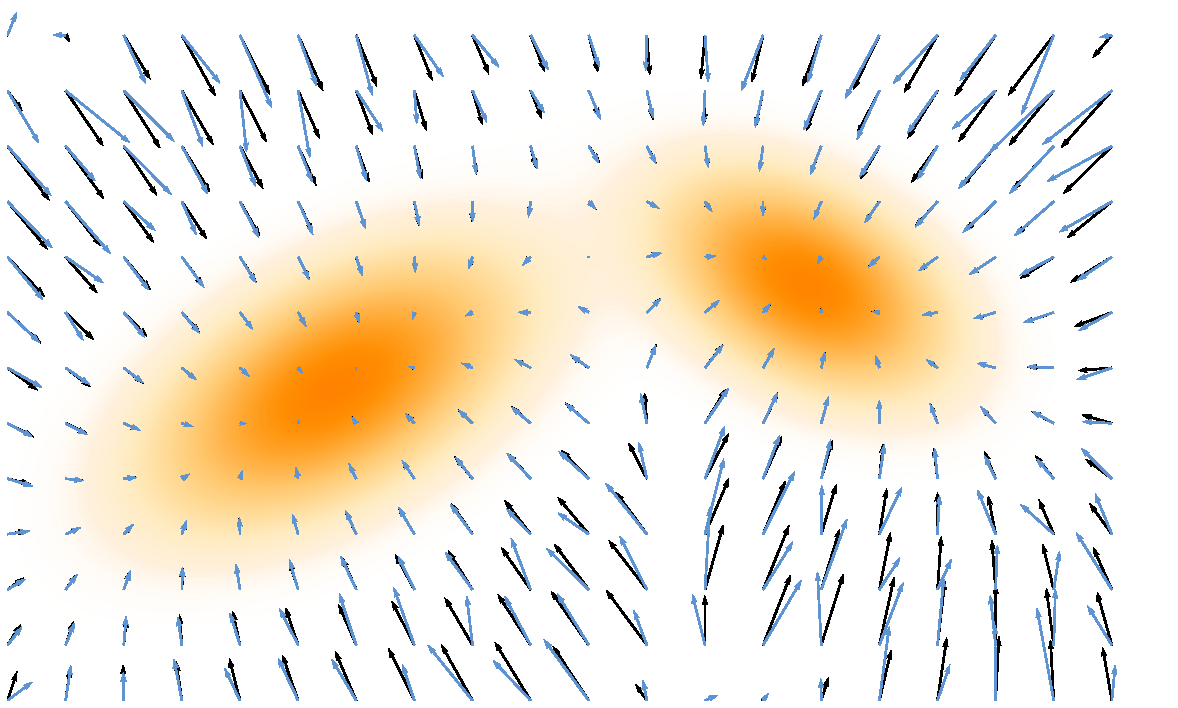
\includegraphics[width=0.9\linewidth]{Images/PartB/score_function_approximation.pdf}
    \caption{\textbfs{分数匹配示意图。} 神经网络分数 ${\color{customblue}\rvs_{\bm{\phi}}(\rvx)}$ 通过 MSE 损失训练以匹配真实分数 $\rvs(\rvx)$。两者都表示为向量场。 \figcredit{由作者绘制。}}
    \label{fig:sm-illustration}
\end{figure}

\subsection{通过分数匹配进行训练}\label{subsec:training-sm}
\paragraph{分数匹配。}
为了从 $p_{\mathrm{data}}$ 的样本中近似分数函数 $\rvs(\rvx) = \nabla_{\rvx} \log p_{\mathrm{data}}(\rvx)$，
我们将其直接近似为由神经网络 $\rvs_{\bm{\phi}}(\rvx)$ 参数化的向量场（见 \Cref{fig:sm-illustration}）：
\[
\rvs_{\bm{\phi}}(\rvx) \approx \rvs(\rvx).
\]
\emph{分数匹配}通过最小化真实分数与估计分数之间的均方误差（MSE）来拟合该向量场：
\begin{mdframed}
\begin{align}\label{eq:sm}
    \mathcal{L}_{\mathrm{SM}}(\bm{\phi}) 
    := \frac{1}{2}  \mathbb{E}_{\rvx \sim p_{\mathrm{data}}}
    \Big[\| \rvs_{\bm{\phi}}(\rvx) - \rvs(\rvx)\|_2^2\Big].
\end{align}
\end{mdframed}

\paragraph{可处理的分数匹配。}
乍看之下，这个目标似乎不可行，因为作为回归目标的真实分数 $\rvs(\rvx)$ 是未知的。
幸运的是，\citet{hyvarinen2005estimation} 证明了分部积分可以得到一个等价目标，它只依赖于模型 $\rvs_{\bm{\phi}}$ 和数据样本，而无需访问真实分数。
我们在下面的命题中陈述这一关键结果：
\proppp{Hyvärinen 的 SM 可处理形式}{sm-trace}
        {
        我们可以将下式表示为：
        \begin{align*}
            \mathcal{L}_{\text{SM}}(\bm{\phi}) = \widetilde{\mathcal{L}}_{\text{SM}}(\bm{\phi}) + C.
        \end{align*}
        其中
        \begin{align}\label{eq:sm-alternative}
            \widetilde{\mathcal{L}}_{\text{SM}}(\bm{\phi})
            := \mathbb{E}_{\rvx \sim p_{\text{data}}(\rvx)} \left[
            \Tr\left(\nabla_{\rvx}\rvs_{\bm{\phi}}(\rvx)\right)
            + \frac{1}{2} \norm{\rvs_{\bm{\phi}}(\rvx)}_2^2
            \right].
        \end{align}
        且 $C$ 是不依赖于 $\bm{\phi}$ 的常数。最小化解 $\rvs^*$ 为：$\rvs^*(\cdot) = \nabla_{\rvx} \log p(\cdot)$。
        }
        {该结果通过展开 $ \mathcal{L}_{\text{SM}} $ 中的 MSE 并应用分部积分得到。证明见 \Cref{app-sec:sm-trace}。
        }

利用 \Cref{eq:sm-alternative} 中的等价目标，我们仅从 $p_{\mathrm{data}}$ 的观测样本训练分数模型 $\rvs_{\bm{\phi}}(\rvx)$，消除了对真实分数函数的需求。


\paragraph{\Cref{eq:sm-alternative} 的直觉。}
替代的分数匹配目标 $\widetilde{\mathcal{L}}_{\text{SM}}(\bm\phi)$
可以直接从它的两项来理解。
范数项 $\tfrac12\|\rvs_{\bm\phi}(\rvx)\|^2$ 在
$p_{\mathrm{data}}$ 较大的区域抑制分数，使这些区域成为驻点。
散度项 $\Tr(\nabla_{\rvx} \rvs_{\bm\phi}(\rvx))$ 在损失中以正号出现，因此最小化该目标会偏好该项取负值。
于是，这些驻点倾向于作为吸引性的汇。
综合来看，该损失将高密度区域塑造成分数场中稳定且收缩的点。
我们在下面详细解释这一点。

\subparagraph{由幅值项得到的驻点性。}
由于 $\widetilde{\mathcal{L}}_{\mathrm{SM}}(\bm\phi)$ 中的期望是在
$p_{\mathrm{data}}$ 下取的，$p_{\mathrm{data}}(\rvx)$ 较大的区域（高数据密度）
对损失的贡献最大。因此幅值项
$\tfrac12\|\rvs_{\bm\phi}(\rvx)\|^2$ 恰恰在这些高概率区域驱动
$\rvs_{\bm\phi}(\rvx)\to 0$，即这些位置变为\emph{驻点}。

\subparagraph{当向量场（近似）为梯度时的凹性。}
由于散度项 $\Tr(\nabla_{\rvx} \rvs_{\bm\phi}(\rvx))$ 以正号进入损失，最小化该目标会促使向量场在高数据密度区域具有负散度。负散度意味着邻近向量会收敛而非散开，因此该区域中的驻点充当\emph{汇}：附近的轨迹被向内牵引。为精确说明这一点，假设
$\rvs_{\bm\phi}=\nabla_{\rvx}u$（其中 $u:\R^D\to\R$ 为标量函数），这在匹配对数密度时是自然的。于是 $\nabla_{\rvx}\rvs_{\bm\phi}=\nabla_{\rvx}^2 u$（Hessian 矩阵）且
$\nabla \cdot \rvs_{\bm\phi}(\rvx)=\Tr(\nabla_{\rvx}^2 u(\rvx))$（散度）。

在驻点 $\rvx_\star$ 处（其中 $\rvs_{\bm\phi}(\rvx_\star)=\nabla_{\rvx}u(\rvx_\star)=\mathbf{0}$），
二阶泰勒展开给出
\[
u(\rvx)
= u(\rvx_\star)
+ \tfrac12(\rvx-\rvx_\star)^\top \nabla_{\rvx}^2 u(\rvx_\star)(\rvx-\rvx_\star)
+ o(\|\rvx-\rvx_\star\|^2).
\]
若 Hessian 矩阵 $\nabla_{\rvx}^2 u(\rvx_\star)$ 负定，则 $u$ 在
$\rvx_\star$ 处局部凹，且对数密度在该处取得严格局部极大值\footnote{我们指出，严格凹性（从而对数密度的严格局部极大值）要求整个 Hessian 矩阵
$\nabla_{\rvx}^2 u$ 负定，而不仅仅迹为负。
负的迹保证了特征值之和为负，但某些特征值仍可能
为正，从而得到鞍点而非极大值。
}。
由于 Hessian 矩阵的所有特征值都为负，迹也为负：
$\Tr(\nabla_{\rvx}^2 u(\rvx_\star))<0$。
因此所学到的向量场具有负散度，该驻点是一个\emph{汇}：微小扰动会被收缩回 $\rvx_\star$。




\subsection{用 Langevin 动力学采样}
一旦通过最小化 \Cref{eq:sm-alternative} 完成训练，分数模型 $\rvs_{\bm{\phi}^\times}(\rvx)$ 就可以在 Langevin 动力学中替代神谕分数进行采样：
\begin{align}\label{eq:score-langevin-emp}
    \mathbf{x}_{n+1} = \mathbf{x}_n + \eta   \rvs_{\bm{\phi}^\times}(\rvx_n) + \sqrt{2\eta}    \bm{\epsilon}_n, \quad \bm{\epsilon}_n \sim \mathcal{N}(\bm{0}, \bm{I}),
\end{align}
其中 $n=0,1,2,\dots$，并以 $\rvx_0$ 初始化。与 EBM 情形 \Cref{eq:continuous-langevin} 一样，该递推恰好是连续时间 Langevin SDE 的 Euler–Maruyama 离散化：
\begin{align*}
    \diff \rvx(t) = \rvs_{\bm{\phi}^\times}(\rvx(t)) \diff t + \sqrt{2} \diff \mathbf{w}(t),
\end{align*}
初始化为 $\rvx(0)$。因此，在小步长极限下，离散与连续表述一致。在实践中，既可以运行离散采样器，也可以直接模拟 SDE。



\subsection{序章：基于分数的生成模型}

在本章余下部分，我们考察分数函数在现代扩散模型中的基础性作用。分数函数最初被引入是为了实现 EBM 的高效训练，如今已演变为新一代生成模型的核心组件。在此基础上，我们探讨分数函数如何为\emph{基于分数的扩散模型}的理论形式和实际实现提供依据，从而为通过随机过程进行数据生成提供一个有原则的框架。


\clearpage
\newpage


\section{\texorpdfstring{去噪分数匹配}{去噪分数匹配}}\label{sec:dsm}

\subsection{动机}
尽管 \Cref{eq:sm-alternative} 中的替代目标
\begin{align*}
    \widetilde{\mathcal{L}}_{\text{SM}}(\bm{\phi}) = \mathbb{E}_{\rvx \sim p_{\mathrm{data}}} \left[\mathrm{Tr}\big(\nabla_{\rvx}\rvs_{\bm{\phi}}(\rvx)\big) + \frac{1}{2} \|\rvs_{\bm{\phi}}(\rvx)\|_2^2 \right]
\end{align*}
更易处理，但它仍然需要计算 Jacobi 矩阵的迹 $\mathrm{Tr}(\nabla_{\rvx}\rvs_{\bm{\phi}}(\rvx))$。虽然这不需要构造完整的 Jacobi 矩阵，但其精确计算通常随输入维度 $D$ 增大而变得更昂贵，因为它需要跨输入坐标汇总导数信息。因此在高维情形下这可能计算代价很高。


为解决此问题，切片分数匹配~\citep{song2020sliced} 用基于随机投影的随机估计来替代迹项。下面我们简要概述其思想。
% \se{perhaps mention huthcinson's trick since they are equivalent}
\paragraph{切片分数匹配与 Hutchinson 估计。} 切片分数匹配通过沿随机``切片''平均方向导数来替代分数匹配中的迹。设 $\rvu\in\R^D$ 是一个\emph{各向同性}随机向量（例如 Rademacher 或标准高斯），满足 $\E[\rvu]=0$ 且 $\E[\rvu\rvu^\top]=\mathbf I$。由 Hutchinson 恒等式
\[
\Tr(\rmA)=\E_{\rvu}[\rvu^\top \rmA \rvu],\quad\text{and}\quad\E_{\rvu}[(\rvu^\top\rvs_{\bphi}(\rvx))^2]=\|\rvs_{\bphi}(\rvx)\|_2^2,
\]
我们得到精确形式
\[
\widetilde{\mathcal{L}}_{\mathrm{SM}}(\bphi)
=\E_{\rvx,\rvu} \Big[\rvu^\top\big(\nabla_{\rvx}\rvs_{\bphi}(\rvx)\big)\rvu+\tfrac12(\rvu^\top\rvs_{\bphi}(\rvx))^2\Big].
\]
这一目标可以通过自动微分高效计算，使用 Jacobi- 和向量-Jacobi- 乘积运算（JVP/VJP），而无需显式计算大型 Jacobi 或 Hessian 矩阵。
对 $K$ 个随机探测取平均得到一个方差为 $\mathcal{O}(1/K)$ 的无偏估计量，
且方向项 $\rvu^\top(\nabla_{\rvx}\rvs_{\bphi})\rvu$ 可以
用 JVP/VJP 例程高效计算而无需显式 Jacobi 矩阵。直观地说，这意味着我们只检查模型在随机方向上的行为：
投影后的分数被推动去对齐更高数据密度的区域，
因此数据点在期望意义下成为驻点。

\paragraph{从切片分数匹配到去噪分数匹配。} 切片分数匹配绕开了 Jacobi 矩阵，但仍然依赖于原始数据分布。
这使其较为脆弱：对于位于低维流形上的图像数据，
分数 $\nabla_{\rvx}\log p_{\mathrm{data}}(\rvx)$ 可能未定义或不稳定，
而且该方法只在观测点处约束向量场，
对其邻域的控制很弱。
它还进一步受到探测引起的方差和重复 JVP/VJP 代价的影响。

我们在此重点关注一种更鲁棒的替代方案——\emph{去噪分数匹配}（DSM）~\citep{vincent2011connection}，
它提供了一种有原则且可扩展的解决方案。



\subsection{训练}
让我们回顾 \Cref{eq:sm} 中的 SM 损失：
\begin{align*}
     \mathcal{L}_{\text{SM}}(\bm{\phi}) =  \frac{1}{2} \mathbb{E}_{\rvx \sim p_{\text{data}}(\rvx)} \left[ \norm{\rvs_{\bm{\phi}}(\rvx) - \nabla_{\rvx} \log p_{\text{data}}(\rvx)}_2^2 \right],
\end{align*}
问题出在难以处理的项 $\nabla_{\rvx} \log p_{\text{data}}(\rvx)$ 上。

\paragraph{\citet{vincent2011connection} 通过条件化给出的解。}
为克服 $\nabla_{\rvx} \log p_{\text{data}}(\rvx)$ 的难以处理性，\citet{vincent2011connection} 提出通过一个尺度为 $\sigma$ 的已知条件分布 $p_{\sigma}(\tilde{\rvx}|\rvx)$ 向数据 $\rvx \sim p_{\text{data}}$ 注入噪声。神经网络 $\rvs_{\bm{\phi}}(\tilde{\rvx}; \sigma)$ 被训练以近似边缘扰动分布
\[
p_\sigma(\tilde{\rvx}) = \int p_{\sigma}(\tilde{\rvx}|\rvx) p_{\text{data}}(\rvx) \diff \rvx
\]
的分数，其方法是最小化损失
\begin{align}\label{eq:sm-noise-loss}
\mathcal{L}_{\text{SM}}(\bm{\phi}; \sigma) := \frac{1}{2} \mathbb{E}_{\tilde{\rvx} \sim p_\sigma} \left[ \norm{\rvs_{\bm{\phi}}(\tilde{\rvx}; \sigma) - \nabla_{\tilde{\rvx}} \log p_\sigma(\tilde{\rvx})}_2^2 \right].
\end{align}

尽管 $\nabla_{\tilde{\rvx}} \log p_\sigma(\tilde{\rvx})$ 通常是难以处理的，但 \citet{vincent2011connection} 证明了以 $\rvx \sim p_{\text{data}}$ 为\emph{条件}可以得到一个等价且可处理的目标——\emph{去噪分数匹配}（DSM）损失：
\begin{mdframed}
\begin{align}\label{eq:dsm-loss}
\mathcal{L}_{\text{DSM}}(\bm{\phi}; \sigma) := \frac{1}{2} \mathbb{E}_{\rvx \sim p_{\text{data}}, \tilde{\rvx} \sim p_{\sigma}(\cdot|\rvx)} \left[ \norm{\rvs_{\bm{\phi}}(\tilde{\rvx}; \sigma) - \nabla_{\tilde{\rvx}} \log p_{\sigma}(\tilde{\rvx}|\rvx)}_2^2 \right].
\end{align}
\end{mdframed}

\Cref{eq:dsm-loss} 的最优最小化解 $\rvs^*$ 满足
\[
\rvs^*(\tilde{\rvx}; \sigma) = \nabla_{\tilde{\rvx}} \log p_\sigma(\tilde{\rvx}),
\]
它对 \Cref{eq:sm-noise-loss} 也是最优的。

例如，当 $p_{\sigma}(\tilde{\rvx}|\rvx)$ 是方差为 $\sigma^2$ 的高斯噪声时，
\[
p_{\sigma}(\tilde{\rvx}|\rvx) = \mathcal{N}(\tilde{\rvx}; \rvx, \sigma^2 \mathbf{I}),
\]
梯度 $\nabla_{\tilde{\rvx}} \log p_{\sigma}(\tilde{\rvx}|\rvx)$ 具有闭式形式（见 \Cref{eq:gaussian-dsm}），使回归目标显式且计算上可处理。

此外，当 $\sigma \approx 0$ 时，$p_\sigma(\tilde{\rvx}) \approx p_{\text{data}}(\rvx)$，且
\[
\rvs^*(\tilde{\rvx}; \sigma) = \nabla_{\tilde{\rvx}} \log p_\sigma(\tilde{\rvx}) \approx \nabla_{\rvx} \log p_{\text{data}}(\rvx),
\]
这表明所学到的分数近似于原始数据分数，从而可以用于生成。

我们在下面的定理中将关于 $\mathcal{L}_{\text{SM}}$ 和 $\mathcal{L}_{\text{DSM}}$ 之间梯度等价性的讨论形式化：
\thmp{$\mathcal{L}_{\text{SM}}$ 与 $\mathcal{L}_{\text{DSM}}$ 的等价性}{sm-dsm}{
对任意固定的噪声尺度 $\sigma > 0$，有：
\begin{align}\label{eq:score-matching}
    \mathcal{L}_{\text{SM}}(\bm{\phi}; \sigma) = \mathcal{L}_{\text{DSM}}(\bm{\phi}; \sigma) + C,
\end{align}
其中 $C$ 是与参数 $\bm{\phi}$ 无关的常数。此外，两个损失的最小化解 $\rvs^*(\cdot; \sigma)$ 满足
\[
    \rvs^*(\tilde{\rvx}; \sigma) = \nabla_{\tilde{\rvx}} \log p_\sigma(\tilde{\rvx}), \quad \text{for almost every } \tilde{\rvx}.
\]
}{等价性由直接计算得到：通过展开 $\mathcal{L}_{\text{SM}}$ 和 $\mathcal{L}_{\text{DSM}}$ 中的 MSE，所有依赖 $\bm{\phi}$ 的项都抵消，只剩下一个与 $\bm{\phi}$ 无关的常数差。\\
 最小化解的推导沿用与命题~\ref{dsm-minimizer} 相同的论证。我们将详细推导推迟到 \Cref{app-sec:sm-dsm}。
}

这个定理与 DDPM 中的定理~\ref{thm:equiv-marginal-kl} 一样，阐明了一个关键的共同原理：
\msg{洞见}{条件化技巧}{条件化技巧也出现在 DDPM 中扩散模型的变分视角中（见定理~\ref{thm:equiv-marginal-kl}），其中以数据点 $\rvx$ 为条件将难以处理的损失转化为可蒙特卡洛估计的可处理损失。类似的思想也出现在基于流的视角中（例如 Flow Matching~\citep{lipman2022flow}），我们将在 \Cref{sec:flow-matching-framework} 中看到。}


\begin{figure}
    \centering
    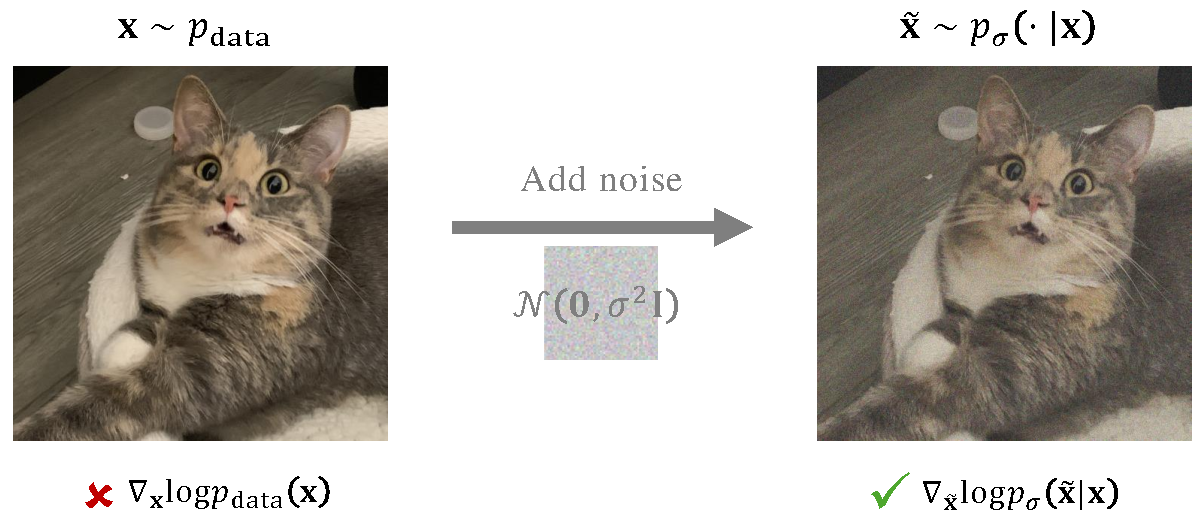
\includegraphics[width=0.8\linewidth]{Images/PartB/dsm-graph.pdf}
    \caption{\textbfs{通过条件化技巧的 DSM 示意图。} 通过用小的高斯加性噪声 $\mathcal{N}(\mathbf{0}, \sigma^2 \rmI)$ 扰动数据分布 $p_{\mathrm{data}}$，所得条件分布 $p_{\sigma}(\tilde{\rvx}|\rvx) = \mathcal{N}(\tilde{\rvx}; \rvx, \sigma^2 \rmI)$ 具有闭式形式的分数函数。
\figcredit{由作者绘制。}}
    \label{fig:dsm-graph}
\end{figure}


\paragraph{特例：加性高斯噪声。} 我们现在考虑常见情形：将方差为 $\sigma^2$ 的高斯噪声 $\mathcal{N}(\mathbf{0}, \sigma^2 \rmI)$ 加到每个数据点 $\rvx \sim p_{\text{data}}$ 上：
\[
\tilde{\rvx} = \rvx + \sigma \bm{\epsilon}, \quad \bm{\epsilon} \sim \mathcal{N}(\mathbf{0}, \rmI),
\]
使得受损数据 $\tilde{\rvx}$ 服从
\[
p_{\sigma}(\tilde{\rvx}|\rvx) = \mathcal{N}(\tilde{\rvx}; \rvx, \sigma^2 \rmI).
\]
在此设置下，条件分数解析地给出为
\[
\nabla_{\tilde{\rvx}} \log p_{\sigma}(\tilde{\rvx}|\rvx) = \frac{\rvx - \tilde{\rvx}}{\sigma^2}.
\]
因此，DSM 损失简化为：
\begin{mdframed}
\begin{align}\label{eq:gaussian-dsm}
\begin{aligned}
    \mathcal{L}_{\text{DSM}}(\bm{\phi}; \sigma) &= \frac{1}{2} \mathbb{E}_{\rvx, \tilde{\rvx}|\rvx} \left[ \norm{\rvs_{\bm{\phi}}(\tilde{\rvx}; \sigma) - \frac{\rvx - \tilde{\rvx}}{\sigma^2}}_2^2 \right] \\
    &= \frac{1}{2} \mathbb{E}_{\rvx, \bm{\epsilon}} \left[ \norm{\rvs_{\bm{\phi}}(\rvx + \sigma \bm{\epsilon}; \sigma) + \frac{\bm{\epsilon}}{\sigma}}_2^2 \right],
\end{aligned}
\end{align}
\end{mdframed}
其中 $\bm{\epsilon} \sim \mathcal{N}(\mathbf{0}, \rmI)$。这一目标构成了（基于分数的）扩散模型的核心。



当噪声水平 $\sigma$ 较小时，高斯平滑的边缘分布
$p_\sigma = p_{\mathrm{data}} * \mathcal{N}(\bm{0},\sigma^2 \rmI)$，
因此它们的高密度区域和分数几乎重合：
$\nabla_{\tilde{\rvx}} \log p_\sigma(\tilde{\rvx}) \approx \nabla_\rvx \log p_{\mathrm{data}}(\rvx)$。
因此，沿带噪分数方向
$\nabla_{\tilde{\rvx}} \log p_\sigma$ 迈出一小步，会将带噪样本移向干净分布本质上相同的高似然区域，
这与 \Cref{subsec:training-sm} 中总结的分数匹配的直觉类似。
相比之下，当 $\sigma$ 较大时，平滑会``过度简化''景观：
$p_\sigma$ 抹平了局部模态，其分数主要把样本拉向全局质量
（想象向均值的收缩），产生可能过度平滑的粗糙去噪。
然而在实践中，DSM 通常假设注入的噪声较小且温和。


为了更好地理解为什么该目标自然对应于一个``去噪''过程，
我们在 \Cref{subsec:why-dsm-denoising-tweedie,subsec:why-dsm-denoising-sure} 中对此讨论进行了展开。


% \se{i think it's important to explain why this is denoising. there's also a reasonable intuition where the best way to denoise is to locally maximize the log-likelihood of the nosy distribution. here it's probably good to at least mention Tweedie's formula, and perhaps Stein's unbiased risk estimator.
% probably worth mentioning that the same idea applies to higher order gradients, and in general to any linear operator
% }



\subsection{采样} 一旦我们在噪声水平 $\sigma$ 下有了训练好的分数模型 $\rvs_{\bm{\phi}^\times}(\tilde{\rvx}; \sigma)$，我们就可以通过用所学模型替代真实分数、用 Langevin 动力学来生成样本。更新规则为：
\begin{align}\label{eq:score-langevin-emp-dsm}
   \tilde{\rvx}_{n+1} = \tilde{\rvx}_n + \eta \underbrace{\rvs_{\bm{\phi}^\times}(\tilde{\rvx}_n; \sigma)}_{\approx \nabla_{\tilde{\rvx}} \log p_\sigma(\tilde{\rvx}_n)} + \sqrt{2\eta}    \bm{\epsilon}_n, \quad \bm{\epsilon}_n \sim \mathcal{N}(\mathbf{0}, \rmI),
\end{align}
其中 $n = 0, 1, 2, \dots$，从初始值 $\tilde{\rvx}_0$ 开始。若 $\sigma$ 足够小，则在足够多次迭代后，$\tilde{\rvx}_n$ 近似于来自 $p_{\text{data}}$ 的样本。


\paragraph{噪声注入的优势。}
我们还要指出，与 \Cref{eq:sm} 中的普通分数匹配相比，注入高斯噪声以形成 $p_\sigma$（例如 \Cref{eq:gaussian-dsm}）具有两个关键优势~\citep{song2019generative}：
\begin{itemize}
  \item \textbfs{良定义的梯度。} 噪声将数据扰动离开其低维流形，得到在 $\mathbb{R}^D$ 上具有完整支撑的分布 $p_\sigma$。因此，分数函数 $\nabla_{\tilde{\rvx}} \log p_\sigma(\tilde{\rvx})$ 处处良定义。
  \item \textbfs{改善的覆盖性。} 噪声平滑了模态之间的稀疏区域，提升了训练信号质量，并使 Langevin 动力学能够更有效地穿越低密度区域。
\end{itemize}


\subsection{为什么 DSM 是去噪：Tweedie 公式}\label{subsec:why-dsm-denoising-tweedie}

我们从\emph{Tweedie 公式}~\citep{efron2011tweedie} 开始，它为仅从带噪观测中进行去噪提供了有原则的基础。
具体而言，它指出：给定来自未知 $\rvx \sim p_{\mathrm{data}}$ 的单个高斯受损观测 $\tilde{\rvx}\sim\mathcal N(\,\cdot\,;\alpha\rvx,\sigma^2\mathrm{I})$，可以通过将 $\tilde{\rvx}$ 沿其带噪边缘分布（定义为下式）的分数
$\nabla_{\tilde{\rvx}}\log p_\sigma(\tilde{\rvx})$ 方向推动大小为 $\sigma^2$ 的一步，得到去噪估计（给定 $\tilde{\rvx}$ 时所有合理干净信号的平均）：
\[
p_\sigma(\tilde{\rvx}):= \int \mathcal{N}(\tilde{\rvx};\alpha \rvx,\sigma^2\mathrm{I})p_{\mathrm{data}}(\rvx)\diff\rvx.
\]
我们在下面正式陈述该命题。
\lemp{Tweedie 公式}{tweedie}{假设 $\rvx\sim p_{\mathrm{data}}$，且在给定 $\rvx$ 的条件下
$\tilde{\rvx}\sim\mathcal N(\,\cdot\,;\alpha\rvx,\sigma^2\mathrm{I})$，其中 $\alpha\neq0$。则 Tweedie 公式表明
 \begin{align}\label{eq:tweedie} 
 \alpha   \mathbb{E}_{\rvx \sim p(\rvx |\tilde\rvx)}\big[\rvx  \big|  \tilde\rvx\big] = \tilde\rvx + \sigma^2 \nabla_{\tilde\rvx} \log p_\sigma(\tilde\rvx), 
 \end{align} 其中期望是在给定 $\tilde\rvx$ 时 $\rvx$ 的后验分布 $p(\rvx |\tilde\rvx)$ 上取的。
}{
证明通过计算边缘分布
$p(\tilde\rvx)=\int p(\tilde\rvx|\rvx)p_{\mathrm{data}}(\rvx)\diff\rvx$ 的分数来完成。
在积分号下求导并利用条件密度的高斯形式，
可以直接得到一个表达式，整理后即得到将分数与后验均值联系起来的恒等式。详见 \Cref{app-sec:tweedie}。
}
Tweedie 公式在扩散模型中起着核心作用，在 DDPM 中引入了多层噪声。
它使得通过分数函数从带噪观测中估计干净样本成为可能，从而在分数预测与去噪器之间建立了一个基本联系：
\begin{equation*}
\underbrace{\mathbb{E} \left[\rvx|\tilde\rvx\right]}_{\substack{\text{denoiser}\\\text{estimated from }\tilde\rvx}}
= \frac{1}{\alpha}\left(\tilde\rvx + \sigma^2 \nabla_{\tilde\rvx} \log p_\sigma(\tilde\rvx)\right).
\end{equation*}

特别地，在带噪对数似然上以特定步长 $\sigma^2$
进行单步梯度上升，就得到去噪估计（条件平均的干净信号）。这使得
DSM 训练与去噪紧密相关：如果由 DSM 训练得到
$\rvs_\bphi(\tilde{\rvx})\approx
\nabla_{\tilde{\rvx}}\log p_\sigma(\tilde{\rvx})$，那么
\[
\frac{1}{\alpha}\left(\tilde{\rvx}+\sigma^2 \rvs_\bphi(\tilde{\rvx})\right)
\]
就是去噪器。

\paragraph{（可选）高阶 Tweedie 公式。} 经典的 Tweedie 公式通过梯度 $\nabla_{\tilde{\rvx}}\log p(\tilde{\rvx})$ 表达后验均值 $\E[\rvx_0|\tilde{\rvx}]$。
高阶扩展~\citep{meng2021estimating} 通过 $\log p(\tilde{\rvx})$ 的高阶导数来表达后验协方差和更高阶累积量。

\subparagraph{带对数归一化因子 $\lambda(\tilde{\rvx})$ 的指数族设置。}
假设给定潜在自然参数 $\boldsymbol\eta\in\R^D$ 时 $\tilde{\rvx}$ 的条件分布属于一个自然指数族，写作
\[
q_\sigma(\tilde{\rvx}|\boldsymbol\eta)
=\exp\!\big(\boldsymbol\eta^\top \tilde{\rvx}-\psi(\boldsymbol\eta)\big)\,q_0(\tilde{\rvx}).
\]
这里 $q_0(\tilde{\rvx})$ 是\emph{基准测度}，即不依赖于 $\boldsymbol\eta$ 的部分；对于方差为 $\sigma^2\rmI$ 的加性高斯噪声它等于 $(2\pi\sigma^2)^{-D/2}\exp(-\|\tilde{\rvx}\|^2/2\sigma^2)$。
设 $p(\boldsymbol\eta)$ 为预先定义的潜在自然参数分布，它可以被视为重新参数化的干净数据分布（对于高斯位置模型，$\boldsymbol\eta=\rvx/\sigma^2$）。
观测到的带噪边缘分布为
\[
p_\sigma(\tilde{\rvx})=\int q_\sigma(\tilde{\rvx}|\boldsymbol\eta)\,p(\boldsymbol\eta)\diff\boldsymbol\eta.
\]
定义 $\tilde{\rvx}$ 处的\emph{对数配分}（对数归一化因子）为
\[
\lambda(\tilde{\rvx}) := \log p_\sigma(\tilde{\rvx})-\log q_0(\tilde{\rvx}).
\]
则给定 $\tilde{\rvx}$ 时 $\boldsymbol\eta$ 的后验为
\[
p(\boldsymbol\eta|\tilde{\rvx})
\ \propto\
\exp\!\big(\boldsymbol\eta^\top \tilde{\rvx}-\psi(\boldsymbol\eta)-\lambda(\tilde{\rvx})\big)\,p(\boldsymbol\eta),
\]
这表明，作为 $\tilde{\rvx}$ 的函数，后验具有指数族形式，其自然参数为 $\tilde{\rvx}$，充分统计量为 $\boldsymbol\eta$，对数配分为 $\lambda(\tilde{\rvx})$。

\subparagraph{$\lambda$ 的导数产生后验累积量。}
这里有两条简单的规则在起作用。
首先是归一化：对每个 $\tilde{\rvx}$，
\[
\int \exp\!\big(\boldsymbol\eta^\top \tilde{\rvx}-\psi(\boldsymbol\eta)-\lambda(\tilde{\rvx})\big)\,p(\boldsymbol\eta)\diff\boldsymbol\eta
=1.
\]
对该恒等式关于 $\tilde{\rvx}$ 求导会从指数项中提取出 $\boldsymbol\eta$ 的各次幂以及 $\lambda(\tilde{\rvx})$ 的导数；将结果置零，就得到 $\lambda$ 的导数与 $\boldsymbol\eta$ 的后验矩之间的等式。
其次是指数族的一个标准性质：对数配分是充分统计量的累积量生成函数。
因此
\[
\nabla_{\tilde{\rvx}}\lambda(\tilde{\rvx})=\E[\boldsymbol\eta|\tilde{\rvx}],\quad
\nabla_{\tilde{\rvx}}^{2}\lambda(\tilde{\rvx})=\Cov[\boldsymbol\eta|\tilde{\rvx}],\quad
\nabla_{\tilde{\rvx}}^{(k)}\lambda(\tilde{\rvx})=\kappa_k(\boldsymbol\eta|\tilde{\rvx})\quad(k\ge 3),
\]
其中 $\kappa_k$ 是给定 $\tilde{\rvx}$ 时随机向量 $\boldsymbol\eta$ 的 $k$ 阶\emph{条件累积量}，通过标准的矩-累积量关系得到。


这些就是高阶 Tweedie 公式。
特化到 $\boldsymbol\eta=\rvx/\sigma^2$ 的高斯位置模型，得到用 $\log p_\sigma(\tilde{\rvx})$ 的导数表示的熟悉形式：
\[
\E[\rvx|\tilde{\rvx}]
=\tilde{\rvx}+\sigma^2\nabla_{\tilde{\rvx}}\log p_\sigma(\tilde{\rvx}),
\qquad
\Cov[\rvx|\tilde{\rvx}]
=\sigma^2\mathrm I+\sigma^4\nabla_{\tilde{\rvx}}^{2}\log p_\sigma(\tilde{\rvx}),
\]
而更高阶的累积量按 $\log p_\sigma(\tilde{\rvx})$ 的高阶导数缩放。


已有若干研究探索了训练神经网络以估计高阶分数~\citep{meng2021estimating,lu2022maximum,lai2023fp}。相比之下，我们的目标是阐明它们与统计量之间的关系，方法论的细节请读者参阅这些工作。

\subsection{（可选）为什么 DSM 是去噪：SURE}\label{subsec:why-dsm-denoising-sure}


\paragraph{SURE（Stein 无偏风险估计）。}
概括地说，Stein 无偏风险估计（SURE）是一种允许在\emph{不知道干净信号}的情况下估计去噪器 $\rmD$ 的均方误差（MSE）的技术。
换言之，SURE 提供了一种在只有带噪数据可用时选择或训练去噪器的方法。

为清晰起见，考虑加性高斯噪声设置：
\[
\tilde{\rvx} = \rvx + \sigma \bm{\epsilon}, 
\qquad \bm{\epsilon} \sim \mathcal{N}(\mathbf{0},\rmI),
\]
其中 $\rvx \in \R^D$ 是未知的干净信号，$\tilde{\rvx}$ 是观测到的带噪版本。
去噪器是任意（弱可微的）映射 $\rmD:\R^D \to \R^D$，它产生 $\rvx$ 的估计 $\rmD(\tilde{\rvx})$。

自然的质量度量是条件 MSE
\[
R(\rmD;\rvx) := \E_{\tilde{\rvx}|\rvx}\left[\|\rmD(\tilde{\rvx})-\rvx\|_2^2 \,\big|\, \rvx\right].
\]
该量依赖于未知的真实值 $\rvx$，因此无法直接计算。
然而，Stein 恒等式（见 \Cref{app-sec:stein-identity}）给出了如下\emph{可观测的}替代量：
\begin{align}\label{eq:sure-obj}
    \mathrm{SURE}(\rmD;\tilde{\rvx})
    = \|\rmD(\tilde{\rvx})-\tilde{\rvx}\|_2^2
    + 2\sigma^2\,\nabla_{\tilde{\rvx}}\cdot \rmD(\tilde{\rvx})
    - D\sigma^2,
\end{align}
其中 $\nabla_{\tilde{\rvx}}\cdot \rmD(\tilde{\rvx})$ 表示 $\rmD$ 的散度。
我们强调，$\mathrm{SURE}(\rmD;\tilde{\rvx})$ 只需要带噪观测 $\tilde\rvx$，而不需要干净的 $\rvx$。

直观上，$\mathrm{SURE}$ 由两个互补的部分组成。
项 $\|\rmD(\tilde{\rvx})-\tilde{\rvx}\|^2$ 度量去噪器输出与带噪输入之间的距离；
单看这一项会低估真实误差，因为 $\tilde{\rvx}$ 已经被污染。
散度项起到修正作用：它刻画了去噪器对其输入微小扰动的敏感程度，
从而有效地把噪声引入的方差考虑在内。


重要的是，对任意固定但未知的 $\rvx$，
\[
\E_{\tilde{\rvx}|\rvx}\left[\mathrm{SURE}(\rmD;\rvx+\sigma\beps) \,\big|\, \rvx\right]
= R(\rmD;\rvx),
\]
其中期望是在高斯噪声 $\beps\sim\mathcal{N}(\bm{0},\rmI)$ 上取的。因此，最小化 SURE（在期望意义下或经验地）等价于最小化真实 MSE，
而只依赖带噪数据。
在实践中，对 $\rvx\sim p_{\mathrm{data}}$ 和污染噪声 $\beps$ 都取平均的 $\mathrm{SURE}$，
给出全局 MSE 风险的无偏估计。

\paragraph{与 Tweedie 公式及 Bayes 最优性的联系。}
设 $p_\sigma(\tilde{\rvx}) = \big(p_{\mathrm{data}} * \mathcal{N}(\mathbf{0}, \sigma^2 \rmI)\big)(\tilde{\rvx})$ 表示本节所考虑的带噪边缘分布。


SURE 是关于噪声（在给定 $\rvx$ 的条件下）的均方误差的无偏估计：
\[
\mathbb{E}_{\tilde{\rvx}| \rvx}\!\big[\mathrm{SURE}(\rmD; \tilde{\rvx})\big]
=
\mathbb{E}_{\tilde{\rvx}| \rvx}\!\big[\|\rmD(\tilde{\rvx})-\rvx\|^2\big].
\]
因此，由全期望定律（塔性质），最小化期望 SURE 等价于最小化 Bayes 风险
$\mathbb{E}_{(\rvx, \tilde{\rvx})}\big[\|\rmD(\tilde{\rvx})-\rvx\|^2\big]
=\mathbb{E}_{\tilde{\rvx}}\!\big[\mathbb{E}_{\rvx| \tilde{\rvx}}\!\big[\|\rmD(\tilde{\rvx})-\rvx\|^2\big]\big]$。这一分解给出了逐点优化：对几乎每个 $\tilde{\rvx}$，
\[
\rmD^*(\tilde{\rvx})
=\arg\min_{\mathbf z}\ \mathbb{E}_{\rvx| \tilde{\rvx}}\!\big[\|\mathbf z-\rvx\|^2\big]
=\mathbb{E}[\rvx| \tilde{\rvx}].
\]
因此，SURE 最优去噪器与 \Cref{subsec:why-dsm-denoising-tweedie} 中的 Bayes 估计量一致，并由 Tweedie 恒等式：
\begin{align}\label{eq:sure-tweedie-denoiser}
    \rmD^*(\tilde{\rvx})=\mathbb{E}[\rvx| \tilde{\rvx}]=\tilde{\rvx}+\sigma^2\nabla_{\tilde{\rvx}}\log p_\sigma(\tilde{\rvx}).
\end{align}




\paragraph{SURE 与分数匹配的关系。}
\Cref{eq:sure-tweedie-denoiser} 中的恒等式促使我们通过分数场来参数化去噪器 $\rmD$：
\[
\rmD(\tilde{\rvx})=\tilde{\rvx}+\sigma^2\rvs_{\bm\phi}(\tilde{\rvx};\sigma),
\]
其中 $\rvs_{\bm\phi}(\cdot;\sigma)$ 旨在近似带噪分数
$\nabla_{\tilde{\rvx}}\log p_\sigma(\cdot)$。
将 $\rmD(\tilde{\rvx})=\tilde{\rvx}+\sigma^2 \rvs_{\bm\phi}(\tilde{\rvx};\sigma)$ 代入 \Cref{eq:sure-obj} 得
\[
\frac{1}{2\sigma^4}\,\mathrm{SURE}(\rmD;\tilde{\rvx})
=
\Tr\!\big(\nabla_{\tilde{\rvx}} s_{\bm\phi}(\tilde{\rvx};\sigma)\big)
+\tfrac12\|\rvs_{\bm\phi}(\tilde{\rvx};\sigma)\|_2^2
+\text{const}(\sigma).
\]
因此，对 $\tilde{\rvx}\sim p_\sigma$ 取期望后，最小化 SURE
等价于（相差一个加性常数）在噪声水平 $\sigma$ 下、在 $p_\sigma$ 下取期望的最小化 Hyvärinen 替代
分数匹配目标（见 \Cref{eq:sm-alternative}）。
因此，两个目标共享相同的最小化解，即 \Cref{eq:sure-tweedie-denoiser} 中的去噪器。



\subsection{（可选）广义分数匹配}


\paragraph{动机。}
经典分数匹配、去噪分数匹配以及高阶变体的目标都是
\[
\frac{\mathcal L p(\rvx)}{p(\rvx)},\quad\text{for some density } p
\]
其中线性算子 $\mathcal L$ 作用于密度。
在经典情形 $\mathcal L=\nabla_{\rvx}$ 下，这给出
\[
\nabla_{\rvx}\log p(\rvx) = \frac{\nabla_{\rvx} p(\rvx)}{p(\rvx)}
\]
$\frac{\mathcal L p}{p}$ 结构允许通过分部积分去除归一化常数，得到一个只依赖于 $p$ 的样本和所学场 $\rvs_\bphi$ 的可处理目标。
这一观点催生了广义分数匹配框架。

\paragraph{广义 Fisher 散度。}
设 $p$ 为数据分布，$q$ 为任意模型分布。
对于作用在 $\rvx$ 的标量函数上的线性算子 $\mathcal L$，定义广义 Fisher 散度
\[
\mathcal D_{\mathcal L}(p \,\|\, q)
:= \int p(\rvx) 
\left\|
\frac{\mathcal L p(\rvx)}{p(\rvx)}
-
\frac{\mathcal L q(\rvx)}{q(\rvx)}
\right\|_2^2 \diff \rvx.
\]
若 $\mathcal L$ 是\emph{完备的}，即
\[
\frac{\mathcal L p_1}{p_1}=\frac{\mathcal L p_2}{p_2} \text{ a.e.}\quad \text{implies}\quad p_1=p_2 \text{ a.e.,}
\]
则 $\mathcal D_{\mathcal L}(p \,\|\, q)=0$ 可确定 $q=p$。
对于 $\mathcal L=\nabla_{\tilde\rvx}$，这恢复为经典 Fisher 散度（见 \Cref{eq:fisher}）。

\paragraph{分数参数化。}
在实践中，我们不对归一化密度 $q$ 建模。
相反，我们直接参数化一个向量场 $\rvs_\bphi(\rvx)$ 来近似广义分数 $\frac{\mathcal L p(\rvx)}{p(\rvx)}$。
考虑
\[
\mathcal D_{\mathcal L}\!\left(p \,\|\, \rvs_\bphi\right)
:= \mathbb E_{\rvx\sim p}\!\left[\left\|\,\rvs_\bphi(\rvx) - \frac{\mathcal L p(\rvx)}{p(\rvx)}\right\|_2^2\right].
\]
尽管 $\frac{\mathcal L p(\rvx)}{p(\rvx)}$ 未知，但``分部积分''使损失只依赖于 $\rvs_\bphi$。
设 $\mathcal L^\dagger$ 为 $\mathcal L$ 的伴随算子，定义为
\[
\int \big(\mathcal L f\big)^\top g
= \int f\,(\mathcal L^\dagger g)
\quad\text{for all test functions } f,g,
\]
当边界项消失时，它在形式上把 $\mathcal L$``移动''到积分另一侧。
展开平方并应用该恒等式，得到可处理的目标
\[
\mathcal L_{\text{GSM}}(\bphi)
= \mathbb E_{\rvx\sim p}\!\left[
\frac{1}{2}\,\|\rvs_\bphi(\rvx)\|_2^2
-
\big(\mathcal L^\dagger \rvs_\bphi\big)(\rvx)
\right] + \text{const},
\]
其中常数不依赖于 $\bphi$。我们只通过期望使用 $p$，因此广义分数匹配损失可以从训练数据得到经验估计量，与经典分数匹配完全一样。

对于 $\mathcal L=\nabla$，有 $\mathcal L^\dagger=-\nabla\!\,\cdot$，这恢复为 \Cref{eq:sm-alternative} 中 Hyvärinen 的分数匹配目标 $\mathbb E_p\!\big[\tfrac{1}{2}\|\rvs_\bphi\|_2^2 + \nabla\!\cdot \rvs_\bphi\big]$。

\paragraph{算子示例。}
\begin{itemize}
\item \textbfs{经典分数匹配。} 考虑 $\mathcal L = \nabla_{\rvx}$。
则广义分数退化为经典分数函数
\[
\frac{\mathcal L p(\rvx)}{p(\rvx)}
= \nabla_{\rvx}\log p(\rvx).
\]
\item \textbfs{去噪分数匹配。}
对于加性高斯噪声，定义算子
\[
(\mathcal L f)(\tilde{\rvx})
= \tilde{\rvx}\,f(\tilde{\rvx}) + \sigma^2\nabla_{\tilde{\rvx}} f(\tilde{\rvx}).
\]
则
\[
\frac{\mathcal L p_\sigma(\tilde{\rvx})}{p_\sigma(\tilde{\rvx})}
= \tilde{\rvx} + \sigma^2\nabla_{\tilde{\rvx}}\log p_\sigma(\tilde{\rvx})
= \mathbb E[\rvx_0|\tilde{\rvx}],
\]
其中 $p_\sigma(\tilde{\rvx}):= \int \mathcal{N}(\tilde{\rvx};\alpha \rvx_0,\sigma^2\mathrm{I})p_{\mathrm{data}}(\rvx)\diff\rvx$ 且 $\tilde\rvx=\rvx+\sigma\beps$。这正是 Tweedie 恒等式。
用该算子最小化 $\mathcal L_{\text{GSM}}$ 会训练 $\rvs_\bphi$ 去近似去噪器，恢复去噪分数匹配目标。


\item \textbfs{高阶目标。}
在 $\mathcal L$ 内部堆叠导数会暴露 $\nabla^2\log p$ 及更高阶导数，它们与后验协方差和高阶累积量对齐。
\end{itemize}


\paragraph{扩展与用例。}
广义分数匹配从连续变量扩展到离散设置，包括语言建模\citep{meng2022concrete,lou2024discrete}。它还启发了产生去噪式目标的、受分数启发的训练。这种算子视角统一了一系列目标，允许从数据进行经验估计，并通过适当选择 $\mathcal L$ 为设计损失函数提供了一般原则.




\clearpage
\newpage


\section{\texorpdfstring{去噪分数匹配的多噪声层级（NCSN）}{去噪分数匹配的多噪声层级（NCSN）}}\label{sec:SMLD}

\subsection{动机}
向数据分布中加入单一固定方差的高斯噪声在一定程度上平滑了它，但只在一个噪声水平上训练基于分数的模型会引入关键局限。在低噪声注入水平下，由于低密度区域的梯度消失，Langevin 动力学难以在多模态分布中穿越模态。相反，在高噪声水平下，采样变得更容易，但模型只能捕捉到粗略结构，导致样本模糊、缺乏精细细节。此外，Langevin 动力学在高维空间中可能收敛缓慢甚至失败。由于它依赖对数密度的梯度进行引导，糟糕的初始化（尤其是在平台区域或鞍点附近）可能阻碍探索，或使采样器被困在单一模态中。


\begin{figure}[ht!]
    \centering
    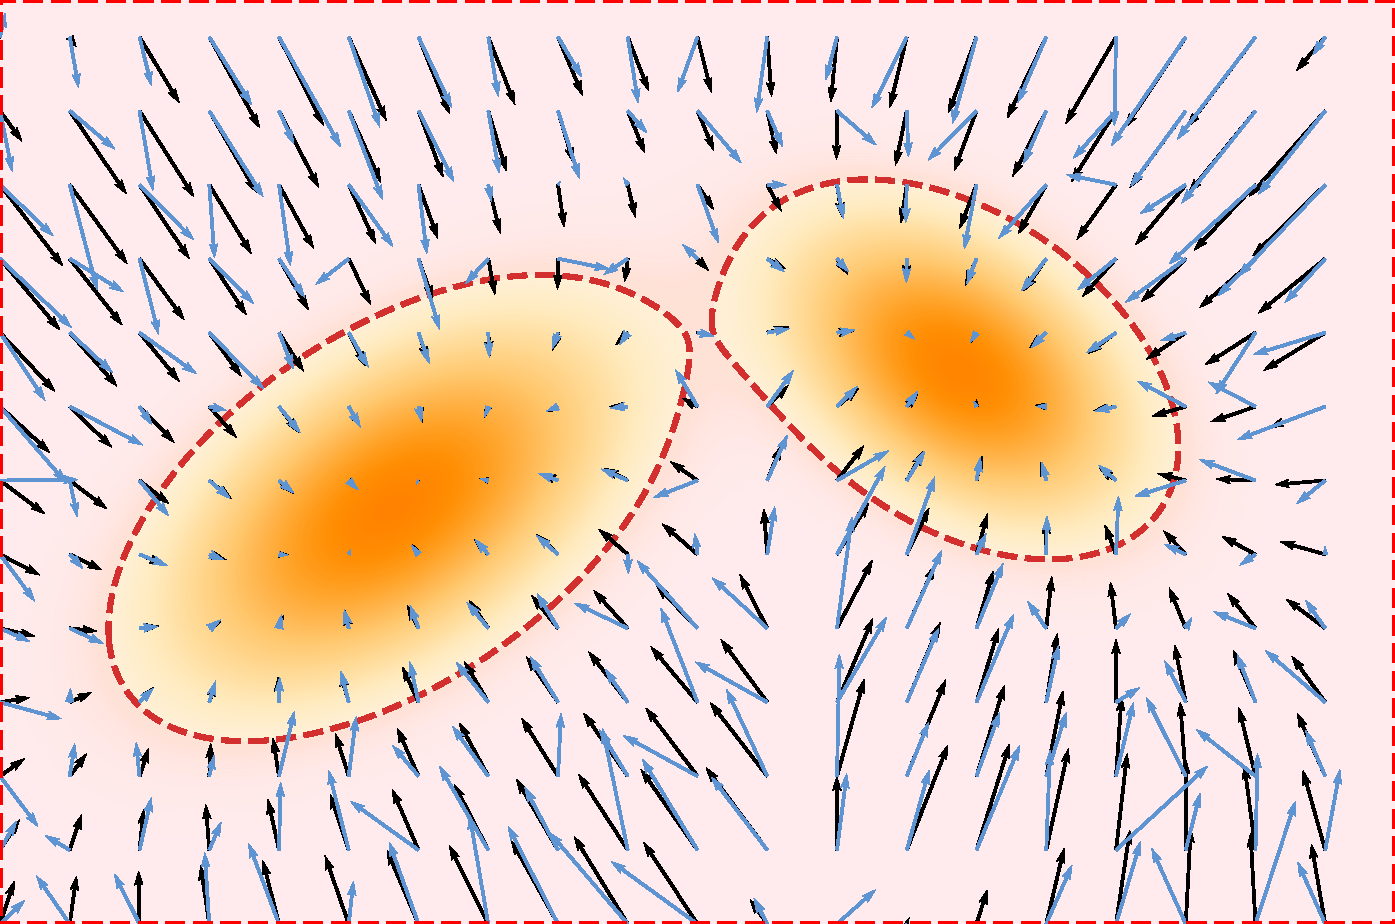
\includegraphics[width=0.85\linewidth]{Images/PartB/score_function_acc.pdf}
    \caption{\textbfs{SM 不准确性的示意图（重访 \Cref{fig:sm-illustration}）。} 红色区域表示由于样本覆盖有限而可能分数估计不准的低密度区域，而高密度区域往往产生更准确的估计。 \figcredit{由作者绘制。}}
    \label{fig:sm-acc-illustration}
\end{figure}


为应对这些挑战，\citet{song2019generative} 提出向数据分布中注入多个水平的高斯噪声，并联合训练一个噪声条件分数网络（NCSN）来估计一系列噪声尺度下的分数函数。在生成时，Langevin 动力学以噪声退火的方式应用：从高噪声水平开始以实现粗略探索，然后逐步细化到低噪声水平以恢复精细细节。




\begin{figure}[th]
    \centering
    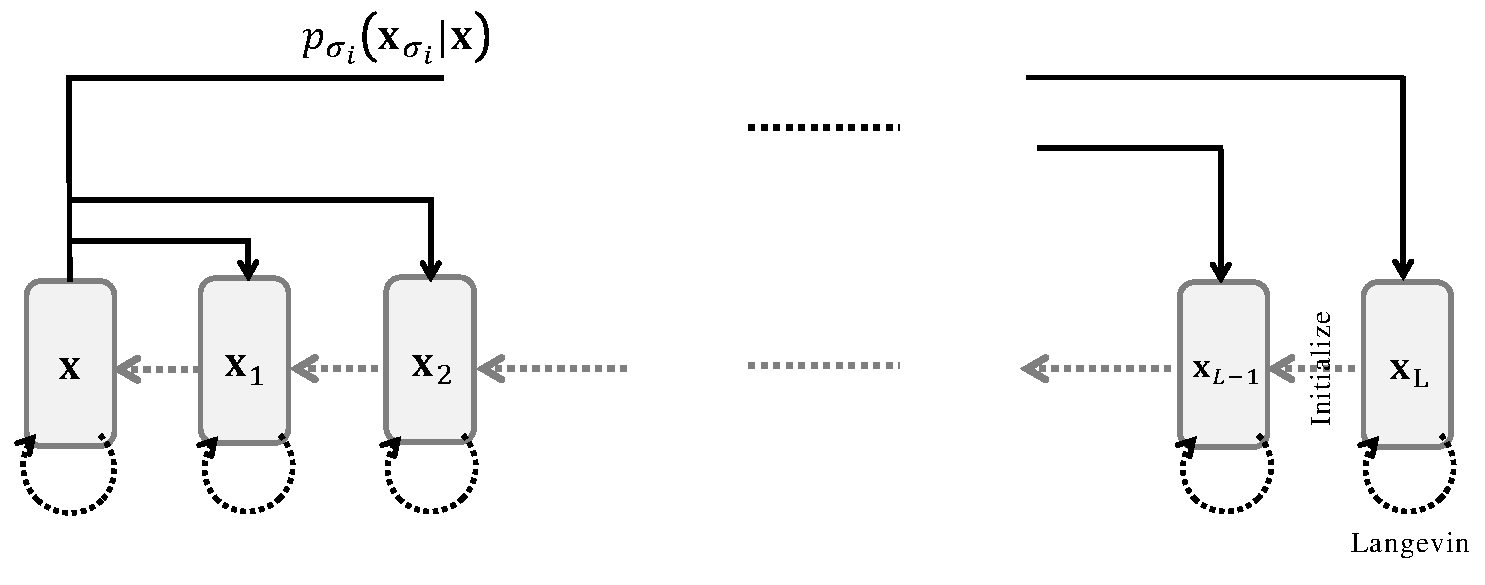
\includegraphics[width=0.95\linewidth]{Images/PartB/ncsn-graph.pdf}
    \caption{\textbfs{NCSN 示意图。} 前向过程用多层加性高斯噪声 $p_{\sigma}(\rvx_{\sigma} | \rvx)$ 扰动数据。生成（虚线）通过在每个噪声层进行 Langevin 采样来进行，并使用当前层的结果作为下一层（更小方差）采样的初始化。 \figcredit{由作者绘制。}}
    \label{fig:smld-ddpm-graphical-model}
\end{figure}


\subsection{训练}
为克服在单一噪声水平上训练基于分数模型的局限，\citet{song2019generative} 提出向数据分布中加入多个水平的高斯噪声。具体地，选择一系列 $L$ 个噪声水平 $\{\sigma_i\}_{i=1}^L$，使得
\[
0 < \sigma_1 < \sigma_2 < \cdots < \sigma_L,
\]
其中 $\sigma_1$ 足够小以保留数据的大部分精细细节，而 $\sigma_L$ 足够大以充分平滑分布，从而便于训练。

每个带噪样本通过扰动干净数据点 $\rvx \sim p_{\text{data}}$ 构造为 $\rvx_{\sigma} = \rvx + \sigma \bm{\epsilon}$，其中 $ \bm{\epsilon} \sim \mathcal{N}(\bm{0}, \rmI)$。这定义了
\vspace{-0.4cm}
\subparagraph{扰动核：}
\[
p_{\sigma}(\rvx_{\sigma} | \rvx) := \mathcal{N}(\rvx_{\sigma}; \rvx, \sigma^2 \rmI),
\]
它诱导出
\vspace{-0.4cm}
\subparagraph{边缘分布：}
\[
p_\sigma(\rvx_{\sigma}) = \int p_{\sigma} (\rvx_{\sigma} | \rvx)    p_{\text{data}}(\rvx) \diff \rvx,
\]
在每个噪声水平 $\sigma$ 处。它表示高斯平滑后的数据分布。

\paragraph{NCSN 的训练目标。}

目标是训练一个噪声条件分数网络 $\rvs_{\bm{\phi}}(\rvx, \sigma)$，以估计所有 $\sigma \in \{\sigma_i\}_{i=1}^L$ 的分数函数 $\nabla_{\rvx} \log p_\sigma(\rvx)$。这是通过在所有噪声水平上最小化 DSM 目标来实现的：
\begin{align}\label{eq:nscn}
\mathcal{L}_{\text{NCSN}}(\bm{\phi}) := \sum_{i=1}^{L} \lambda(\sigma_i)   \mathcal{L}_{\text{DSM}}(\bm{\phi}; \sigma_i),
\end{align}
其中
\begin{align*}
\mathcal{L}_{\text{DSM}}(\bm{\phi}; \sigma) 
= \frac{1}{2} \mathbb{E}_{\rvx \sim p_{\text{data}}(\rvx),   \tilde{\rvx} \sim p_{\sigma}(\tilde{\rvx} | \rvx)} 
\left[ \norm{\rvs_{\bm{\phi}}(\tilde{\rvx}, \sigma) - \left( \frac{\rvx - \tilde{\rvx}}{\sigma^2} \right)}_2^2 \right],
\end{align*}
且 $\lambda(\sigma_i)>0$ 是每个尺度的加权函数。

最小化该目标得到分数模型 $\rvs^*(\rvx, \sigma)$，它在每个噪声水平恢复真实分数：
\[
\rvs^*(\cdot, \sigma) = \nabla_{\rvx} \log p_\sigma(\cdot),  \quad \text{for all } \sigma \in \{\sigma_i\}_{i=1}^L,
\]
因为它本质上是 DSM 最小化（见定理~\ref{thm:sm-dsm}）。
% \se{discuss replationship with ddpm loss}


\paragraph{与 DDPM 损失的关系。}
设 $\rvx_\sigma=\rvx+\sigma\boldsymbol{\epsilon}$，其中 $\boldsymbol{\epsilon}\sim\mathcal{N}(\mathbf{0},\mathbf{I})$，并设 $p_\sigma$ 表示边缘分布。由 Tweedie 公式，
\[
\nabla_{\rvx_\sigma}\log p_\sigma(\rvx_\sigma)
= -\frac{1}{\sigma} \E \left[\boldsymbol{\epsilon} \middle|  \rvx_\sigma\right].
\]
因此 NCSN 的最优解是真实分数 $\rvs^*(\rvx_\sigma,\sigma)=\nabla_{\rvx_\sigma}\log p_\sigma(\rvx_\sigma)$，而 DDPM 损失 \Cref{eq:ddpm-simple-loss} 下的 Bayes 最优噪声预测器是 $\boldsymbol{\epsilon}^*(\rvx_\sigma,\sigma)=\E[\boldsymbol{\epsilon}|\rvx_\sigma]$。它们通过下式完全等价
\[
\rvs^*(\rvx_\sigma,\sigma) = - \frac{1}{\sigma} \boldsymbol{\epsilon}^*(\rvx_\sigma,\sigma),
\qquad
\boldsymbol{\epsilon}^*(\rvx_\sigma,\sigma) = - \sigma \rvs^*(\rvx_\sigma,\sigma).
\]
在 DDPM 的扰动 \Cref{eq:ddpm-perturbation}（离散指标 $i$）中，
\[
\rvx_i = \bar{\alpha}_i \rvx_0 + \sqrt{1 - \bar{\alpha}_i^2}
\]
同一关系给出
\[
\rvs^*(\rvx_i,i)= -\frac{1}{\sigma_i} \E \left[\boldsymbol{\epsilon} \middle|  \rvx_i\right],
\]
因此最小化 \Cref{eq:ddpm-simple-loss} 学习的是 $\boldsymbol{\epsilon}$ 的条件去噪器，它是噪声水平 $i$ 处真实分数的一个带缩放的重新参数化。

我们将在 \Cref{ch:all-equivalent} 中系统地比较和总结这种参数化的等价性。



\subsection{采样} 
\begin{algorithm}[th]
\caption{\label{alg:smld} 退火 Langevin 动力学}
\begin{algorithmic}[1]
\Require 已训练的分数 $\rvs_{\bm{\phi}^\times}(\cdot, \sigma_\ell)$、步长 $\eta_\ell$ 以及每个噪声水平 $\ell = L, \dots, 2$ 的 Langevin 迭代预算 $N_\ell$
\State $\rvx^{\sigma_L} \sim \mathcal{N}(\mathbf{0}, \mathbf{I})$
\For{$\ell = L, \dots, 2$}
    \State $\tilde{\rvx}_0 \gets \rvx^{\sigma_\ell}$
    \Statex\Comment{用上一噪声层的输出初始化 Langevin}
    \For{$n = 0$ \textbf{to} $N_\ell - 1$}
        \State $\bm{\epsilon}_n \sim \mathcal{N}(\mathbf{0}, \mathbf{I})$
        \State $\tilde{\rvx}_{n+1} \gets \tilde{\rvx}_n + \eta_\ell \rvs_{\bm{\phi}^\times}(\tilde{\rvx}_n, \sigma_\ell) + \sqrt{2\eta_\ell} \bm{\epsilon}_n$
    \EndFor
    \State $\rvx^{\sigma_{\ell-1}} \gets \tilde{\rvx}_{N_\ell}$
    \Statex \Comment{输出用作下一噪声层的初始化}
\EndFor
\Ensure $\rvx^{\sigma_1}$ 
\end{algorithmic}
\end{algorithm}


在多个噪声水平上都有训练好的分数网络后
\[
\rvs_{\bm{\phi}^\times}(\cdot, \sigma_1), \quad\rvs_{\bm{\phi}^\times}(\cdot, \sigma_2), \quad \cdots, \quad \rvs_{\bm{\phi}^\times}(\cdot, \sigma_{L-1}), \quad    \rvs_{\bm{\phi}^\times}(\cdot, \sigma_L),
\]
% \se{this notation is weird}\jcc{do you meant the notation of $\bm{\phi}^\times$ is weird, which i was thoroughly using $\bm{\phi}^\times$ to denote a trained network? }
被称为\emph{退火 Langevin 动力学}~\citep{song2019generative} 的采样过程通过从高噪声水平 $\sigma_L$ 逐步去噪到低噪声水平 $\sigma_1 \approx 0$ 来生成数据。

从高斯噪声 $\rvx^{\sigma_L} \sim \mathcal{N}(\bm{0}, \rmI)$ 开始，该算法在每个噪声水平 $\sigma_\ell$ 应用 Langevin 动力学，以近似地从扰动分布 $p_{\sigma_\ell}(\rvx)$ 中采样。$\sigma_\ell$ 层的输出用于为下一个更低噪声水平 $\sigma_{\ell-1}$ 提供\emph{更好的初始化}。

在每个水平，Langevin 动力学迭代地更新：
\[
\tilde{\rvx}_{n+1} = \tilde{\rvx}_n + \eta_\ell \rvs_{\bm{\phi}^\times}(\tilde{\rvx}_n, \sigma_\ell) + \sqrt{2\eta_\ell} \bm{\epsilon}_n, \quad \bm{\epsilon}_n \sim \mathcal{N}(\bm{0}, \rmI),
\]
从 $\tilde{\rvx}_0 := \rvx^{\sigma_\ell}$ 开始。步长通常按噪声水平缩放：
\[
\eta_\ell = \delta \cdot \frac{\sigma_\ell^2}{\sigma_1^2}, \quad \text{for some fixed } \delta > 0.
\]
这种噪声退火的细化一直进行到最低噪声水平 $\sigma_1$，在那里得到最终样本 $\rvx^{\sigma_1}$。通过逐步地把上一层的输出作为下一层更好的初始化，这一策略实现了对复杂数据分布更有效的探索和更优的覆盖。\Cref{alg:smld} 总结了该过程。

\paragraph{NCSN 采样速度慢。}
NCSN 使用退火 MCMC（通常是 Langevin 动力学）跨噪声尺度 $\{\sigma_i\}_{i=1}^L$ 生成样本。
对每个尺度 $\sigma_i$，它执行 $K$ 次``用分数 $\rvs_{\bm{\phi}^\times}(\tilde{\mathbf{x}}_n,\sigma_i)$ 加上一个小随机扰动来更新 $\tilde{\mathbf{x}}_n$''形式的迭代更新，每次都需要通过分数网络的一次前向传播。两个因素使得 $L \times K$ 必须很大：
\begin{enumerate}
    \item[(i)] \textbfs{局部精度与稳定性：} 所学到的分数只对小扰动可靠，需要小步长和每个噪声水平多次迭代以避免偏差或不稳定；
    \item[(ii)] \textbfs{高维下混合缓慢：} 局部 MCMC 移动低效地探索多模态、高维目标，需要大量迭代才能到达典型数据区域。
\end{enumerate}
由于更新严格串行（每次迭代依赖于前一次），且每次都需要昂贵的网络计算，总代价是 $\mathcal{O}(L  K)$ 次串行网络传播，使采样在计算上很慢。

% \newpage

% \paragraph{Link Between Fisher Divergence and KL Divergence.} Maximum likelihood fits $q_\bphi$ by minimizing $\mathcal{D}_\mathrm{KL}(p\|q_\bphi)=\mathbb{E}_{p}[\log p-\log q_\bphi]$. Score matching fits $q_\bphi$ by minimizing the Fisher divergence $\mathcal{D}_{\mathrm F}(p\|q_\bphi)=\mathbb{E}_{p} \big[\|\nabla \log p-\nabla \log q_\bphi\|^2\big]$. They agree at the optimum ($p=q_\bphi$) but use different discrepancy measures. The key bridge is that when you smooth both distributions with Gaussian noise, $p_t=p*\mathcal N(\bm{0},t\rmI)$ and $q_t=q_\bphi*\mathcal N(\bm{0},t\rmI)$, the KL decreases along the noise scale at a rate given by Fisher:
% \[
% \frac{\diff}{\diff t}\mathcal{D}_\mathrm{KL}(p_t\|q_t)=-\tfrac12 \mathcal{D}_{\mathrm F}(p_t\|q_t).
% \]
% So Fisher is the instantaneous decay rate of KL under Gaussian smoothing. Moreover, for many smooth, near Gaussian targets (those satisfying a log Sobolev inequality), minimizing $\mathcal{D}_{\mathrm F}(p\|q_\bphi)$ controls $\mathcal{D}_\mathrm{KL}(p\|q_\bphi)$ via a bound like $\mathcal{D}_\mathrm{KL}(p\|q_\bphi)\lesssim \mathcal{D}_{\mathrm F}(p\|q_\bphi)$. In practice, this explains why score matching (and its denoising version used in diffusion models) can learn models with good likelihood while avoiding the intractable partition function: it matches scores directly, which do not depend on normalization, yet it still pushes down KL through the smoothing identity.



\clearpage
\newpage

\section{小结：NCSN 与 DDPM 的比较视角}

我们首先在 \Cref{fig:smld-ddpm-graphical-model} 中比较 NCSN 和 DDPM 的图模型，关键异同总结在 \Cref{tb:comparison-smld-ddpm} 中。


\begin{table}[th]
  \caption{NCSN 与 DDPM 的比较}
  \small
  \centering
  \resizebox{\textwidth}{!}{
  \begin{tabular}{cccc}
     \toprule
    
         &   \textbfs{NCSN}   & \textbfs{DDPM}  \\
        \midrule
    $\rvx_{i+1}|\rvx_{i}$ & 推导为 $\rvx_{i+1} =  \rvx_i + \sqrt{\sigma^2_{i+1}-\sigma^2_{i}}\bm{\epsilon}$   &  \cc{15}定义为 $\rvx_{i+1} = \sqrt{1-\beta_{i}} \rvx_{i} + \sqrt{\beta_{i}}\bm{\epsilon}$  \\
      $\rvx_{i}|\rvx$   & \cc{15}定义为 $\rvx_{i} =  \rvx + \sigma_{i}\bm{\epsilon}$
       &  推导为 $\rvx_i = \bar{\alpha}_i\rvx + \sqrt{1 - \bar{\alpha}_i^2}\bm{\epsilon}$ \\
   $p_{\text{prior}}$   & $ \mathcal{N}(\bm{0}, \sigma_L^2\rmI)$    &  $\mathcal{N}(\bm{0}, \rmI)$  \\
   \midrule
        损失 
          &  
        $\mathbb{E}_{i} \mathbb{E}_{p_{\text{data}}(\rvx)} 
        \mathbb{E}_{\bm{\epsilon} \sim \mathcal{N}\left(\mathbf{0}, \rmI\right)}   
    \left[ \norm{\rvs_{\bm{\phi}}(\rvx_i, \sigma_i) +   \frac{\bm{\epsilon}}{\sigma_i}}_2^2 \right] $ 
            &  $      \mathbb{E}_{i}\mathbb{E}_{p_{\text{data}}(\rvx)} \mathbb{E}_{\bm{\epsilon}\sim \mathcal{N}(\bm{0},\rmI)}\left[ \norm{\bm{\epsilon}_{\bm{\phi}}(\rvx_i, i) - \bm{\epsilon}}_2^2 \right]$ \\
    \midrule
     采样   & \begin{tabular}{@{}c@{}} 逐层应用 Langevin 动力学；\\ 用输出初始化下一层 \end{tabular}  &  \begin{tabular}{@{}c@{}}沿马尔可夫链遍历 \\ $p_{\bm{\phi}^\times}(\rvx_{i-1} | \rvx_i)$   \end{tabular} \\
 \bottomrule
  \end{tabular}
  }
  \label{tb:comparison-smld-ddpm}
\end{table}

\paragraph{共同的瓶颈。}
尽管形式不同，NCSN 和 DDPM 都依赖于密集的时间离散化。这导致一个关键局限：采样往往需要数百甚至数千次迭代，使生成缓慢且计算密集。

\begin{question}\label{ques:dm-sampling-slow}
    我们如何加速扩散模型中的采样？
\end{question}

我们在 \Cref{ch:solvers}（开发更高效的采样器）、\Cref{ch:distillation}（将需要数百采样步骤的预训练扩散模型压缩为更少步骤的学生生成器）以及 \Cref{ch:fast-scratch}（研究如何在扩散启发的原则下直接从头学习快速的少步生成器）中回到这一挑战。

% \paragraph{What Lies Ahead?}

% Despite their seemingly different origins, NCSN and DDPM share a strikingly similar high-level philosophy. Both inject noise at multiple levels and train models to progressively denoise, enabling tractable learning through conditioning and effective generation via noise-annealed refinement. This principle of layering stochasticity and learning to reverse it step-by-step provides a powerful foundation for modeling complex data distributions. 

% In the next chapter, \Cref{ch:score-sde}, we step into the continuous-time world, where the boundary between DDPM and NCSN begins to blur, revealing a profound unification at the heart of diffusion modeling.

\newpage

\section{结语}\label{sec:ch3_cr}



本章勾勒了通向扩散模型的第二条主要路径，起点是根植于基于能量的模型（EBM）的分数视角。我们从识别 EBM 的核心挑战——难以处理的配分函数——开始，并引入分数函数 $\nabla_{\mathbf{x}}\log{p(\mathbf{x})}$ 作为完全绕开这一问题的有力工具。

我们的旅程从经典分数匹配走向其更具可扩展性和鲁棒性的变体——去噪分数匹配（DSM）。通过 DSM，我们看到了用噪声扰动数据如何带来可处理的训练目标，再次利用条件化策略来创建简单的回归目标。此外，我们通过 Tweedie 公式建立了分数估计与去噪行为之间的深刻联系，它表明分数提供了从带噪观测中估计干净信号所需的精确方向。


这一原理随后从单一噪声水平扩展到由噪声条件分数网络（NCSN）构成的连续体，NCSN 学习一个以多个噪声尺度为条件的单一分数模型，并通过退火 Langevin 动力学生成样本。在探索结束时，我们发现 NCSN 与来自变分视角的 DDPM 尽管起源不同，却共享惊人相似的结构和一个共同的瓶颈：缓慢的串行采样。



这种收敛并非巧合；它暗示着一种更深层的、统一的数学结构。这些离散时间模型的局限促使我们需要一个更一般的框架。在下一章中，我们将迈出这关键一步：
\begin{enumerate}
    \item 我们将进入连续时间视角，证明 DDPM 和 NCSN 都可以优雅地统一为由随机微分方程（SDE）描述的单一强大过程的不同离散化。
    \item 这一 Score SDE 框架将正式连接变分视角与基于分数的视角，把生成问题重新表述为求解微分方程的问题。
\end{enumerate}

这一统一视角不仅将提供深刻的理论清晰度，还将开启一类旨在解决采样缓慢这一根本挑战的先进数值方法。